%%%%%%%%%%%%%%%%%%%%%%%%%%%%%%%%%%%%%%%%%%%%%%%%%%%
%%%%%%%%%%%%%%%%%%%%%%%%%%%%%%%%%%%%%%%%%%%%%%%%%%%
%%
%%       Report of the analyzing for Hadoop
%%
%%       Copyright (C) XDUSakura 2017
%%
%%       <pari passu>
%%       李约瀚 (John Lee) (Qinka) <qinka@live.com> <me@qinka.pro>
%%       康赣鹏
%%       乔新文 (Xinwen Qiao) (starsriver) <starsriver@outlook.com>
%%       罗赛男
%%       杨瑞
%%
%%
%%%%%%%%%%%%%%%%%%%%%%%%%%%%%%%%%%%%%%%%%%%%%%%%%%%
%%%%%%%%%%%%%%%%%%%%%%%%%%%%%%%%%%%%%%%%%%%%%%%%%%%

%% 使用 XeTeX 编译


% 使用 CTeX 的 Report 模版
\documentclass{ctexart}

%% 导言区
%% 所有需要添加的宏包,先创建新分支然后测试,最后等待负责的人,合并到主开发分支
%% 首先从 dev/base 牵出一个新的分支,加上所需要增加的导言区,然后再从此处牵出另一个新分支
%% 并与所需要导言区的代码部分进行合并,并测试,测试成功之后,将第二次添加的分支删去
%% 第一次添加的分支等待被合并回 dev/base 分支
%% 然后其他再根据邮件活着其他的内容进行合并

%% 用于处理交叉引用并提供超链接
%% CTAN: https://www.ctan.org/pkg/hyperref
\usepackage{hyperref}

%% 用于处理代码,显示代码的
%% CTAN: https://www.ctan.org/pkg/listings
\usepackage{listings}
%% 配置 样式
\lstset{ breaklines %% 控制换行
       , numbers=left %% 在左边显示行号
       }
%% 定义 Java 代码环境
\lstnewenvironment{java}[1][]
{ \lstset{#1%
    }%
  \csname lst@SetFirstLabel\endcsname}
{ \csname lst@SaveFirstLabel\endcsname}


%% 导言区结束

%% 报告标题
\title{Analyzation of Hadoop's File System \\ Hadoop 文件系统代码分析报告}
%% 作者
\author{李约瀚 \\ 14130140331 \\ qinka@live.com \\ me@qinka.pro %
   \and 康赣鹏 \\ 14130140xxx \\ email@domain%
   \and 乔新文 \\ 141301400393 \\ starsriver@outlook.com %
   \and 罗赛男 \\ 14130140363 \\ luosainan96@163.com%
   \and  杨瑞  \\ 14130140xxx \\ email@domain%
   % 格式 姓名 【换行】 学号 【换行】 邮箱 【换行】 邮箱 (可以只有一个。。。
   }

\begin{document}
    \maketitle
    \newpage
    \tableofcontents
    \newpage

    %% 摘要
    

%% 结束
\endinput
    %% 环境
    \section{Environment}
\label{sec:environment}

Hadoop 发展到今天,整个项目已经不能简单的用“庞大”这样的词语来形容了。运行 Hadoop 的环境通常需要配置很久,
虽然依赖 Java 的跨平台的特性, Hadoop 在不同平台上移植不是难事,然而部署却需要花费不少功夫。
通常的步骤是先编写一堆配置文件,然后初始化 HDFS, 最后验证并启动 Hadoop。
好在 Hadoop 官方提供了 Dockerfile, 能比较容易的将 Hadoop 打包成 Docker镜像,然后运行。

代码分析使用的是 Hadoop 2.8.0 的源代码,代码是从官方在 GitHub 上的仓库 fork 出来的。
同时还运用到了 StartUML 等工具绘制 UML 类图等。

%% 结束
\endinput
    %% SA
    \section{Software Architecture}
\label{sec:sa}


%% 结束
\endinput
    %% UML
    \section{??}
\label{sec:UML}

%% inputstream
%% 结束
\subsection{InputStream 代码分析}
	\subsubsection{IntputStream类结构层次} 
	整个InputStream中大部分都在讲本地文件的读写,只有少部分关于dfs,也就是分布式文件系统。整个InputStream一条继承链和好多接口,其中FSDataInputStream实现了大部分接口。InputStream 为字节输入流,它本身为一个抽象类,基于字节的输入操作,此抽象类是表示字节输入流的所有类的超类。定义了所有输入流都具有的共同特征。必须依靠其子类实现各种功能。如图 \ref{fig:graph1} 所示
	
	\begin{figure}
		\centering
	    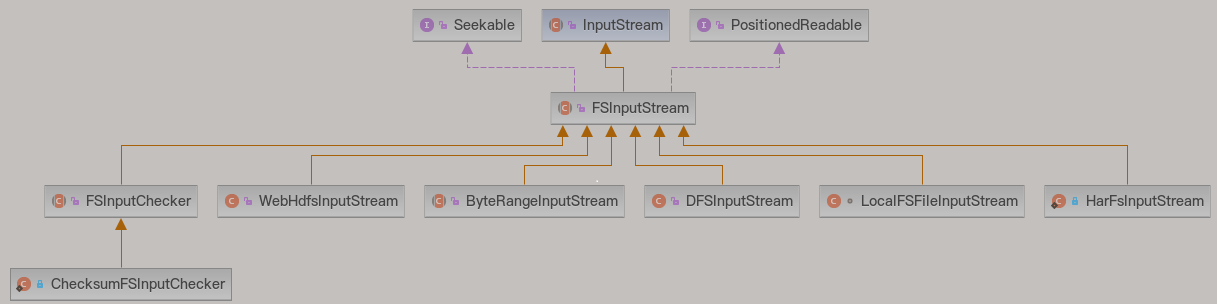
\includegraphics[width=3in,height=3in]{UML/inputstream/hdfs-common-inputstream-diagram.png}
		\caption{IntputStream类结构层次}
		\label{fig:graph1}
	\end{figure}
	
	\subsubsection{IntputStream类结构分析} 
	Java的IO模型设计非常优秀,它使用Decorator模式,按功能划分Stream,我们可以动态装配这些Stream,以便获得您需要的功能。例如,我们需要一个具有缓冲的文件输入流,则应当组合使用FileInputStream和BufferedInputStream。另外简单数一下Java IO中的装饰模式:在IO中,具体构件角色是节点流,装饰角色是过滤流。FilterInputStream和FilterOutputStream是装饰角色,而其他派生自它们的类则是具体装饰角色。如图\ref{fig:graph2} 所示
	
	\begin{figure}
		\centering
		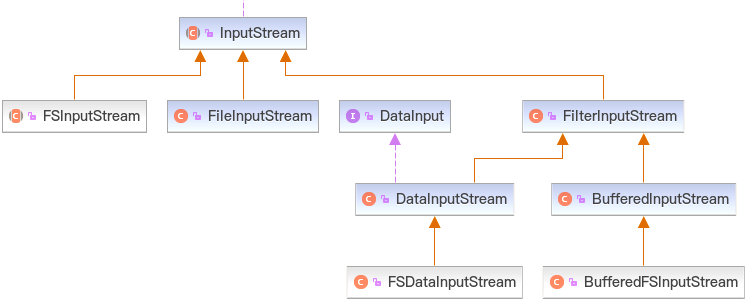
\includegraphics[width=3in,height=3in]{UML/inputstream/common-io-diagram.png}
		\caption{IntputStream部分类}
		\label{fig:graph2}
	\end{figure}
	
	\subsubsection{FSInputStream}
	FSInputStream 实现了接口 Seekable 和 PositionedReadable。提供了基本的读取一个输入流的操作,比如定位seek和读取到特定的buffer的操作read和readFully。FSInputStream在原有InputStream 基础之上添加了 getPos 方法,同时可以通过 seek 方法定位指定的偏移量处。新添加的 getPos 和 seek 方法在 FSDataInputStream 类中被使用。如图\ref{fig:graph3} 和 \ref{fig:graph4}所示
	
	\begin{figure}
		\centering
		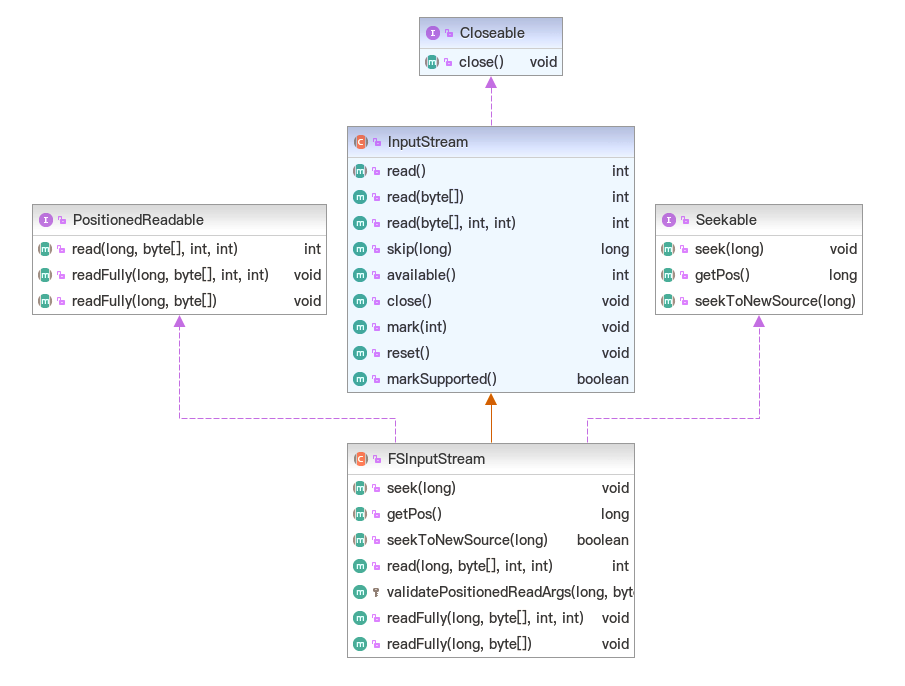
\includegraphics[width=3in,height=3in]{UML/inputstream/hdfs-fsinputstream-methods-diagram.png}
		\caption{hdfs-fsinputstream-methods-diagram}
		\label{fig:graph3}
	\end{figure}
	\begin{figure}
		\centering
		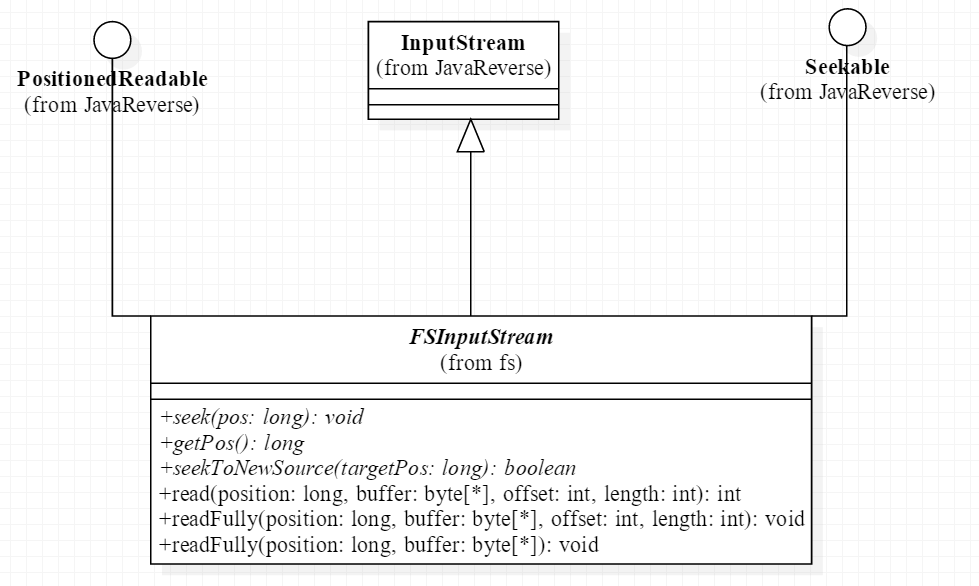
\includegraphics[width=3in,height=3in]{UML/inputstream/UML.png}
		\caption{FSInputStream类和接口}
		\label{fig:graph4}
	\end{figure}
	
	\subsubsection{PositionedReadable}
	\begin{figure}
		\centering
		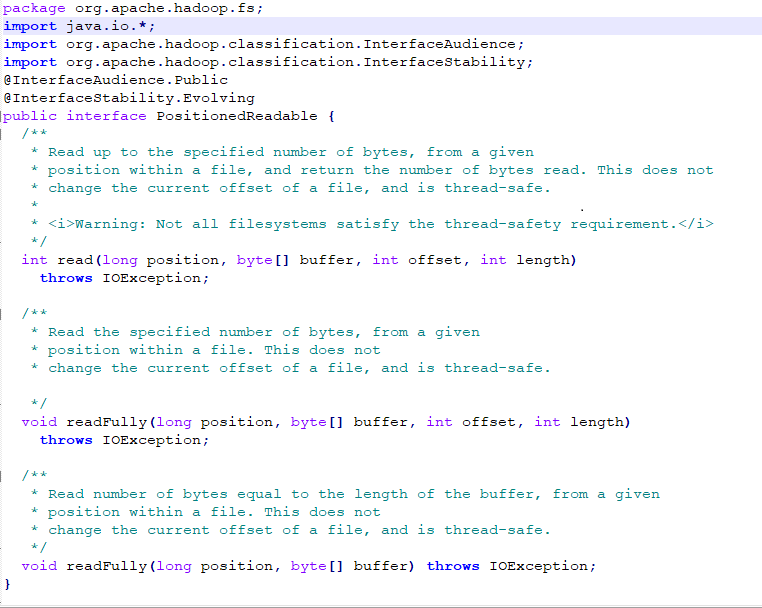
\includegraphics[width=3in,height=3in]{UML/inputstream/PositionedReadable.png}
		\caption{PositionedReadable}
		\label{fig:graph5}
	\end{figure}
	
	
	 \subsubsection{Seekable}

	\begin{figure}
		\centering
		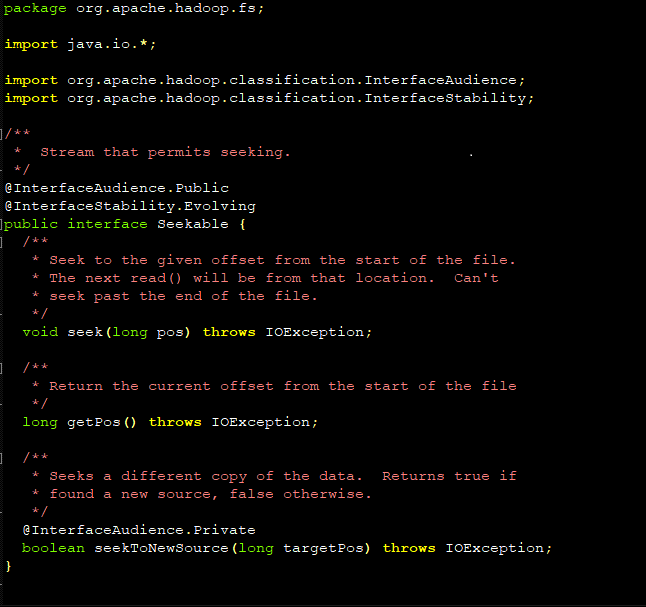
\includegraphics[width=3in,height=3in]{UML/inputstream/Seekable.png}
		\caption{Seekable}
		\label{fig:graph6}
	\end{figure}
	
	\subsubsection{FSInputChecker}
	FSInputChecker 提供了检测校验和的功能,主要实现了 read 方法。在 read 方法中调用了 read1方法。每当读取的数据字节数大于 maxChunkSize 时,就会调用 readChecksumChunk 方法。在readChecksumChunk 方法中,进一步调用 readChunk 抽象方法来实现真正的数据读取。读取完数据后,然后判断是否需要检验校验和,如果需要,则调用 private void verifySums(final byte b[], final int off, int read)throws ChecksumException 进行检验,如果有错,则抛出异常。abstract protected int readChunk(long pos, byte[] buf, int offset, int len,byte[] checksum) throws IOException;
	
	\begin{figure}
		\centering
		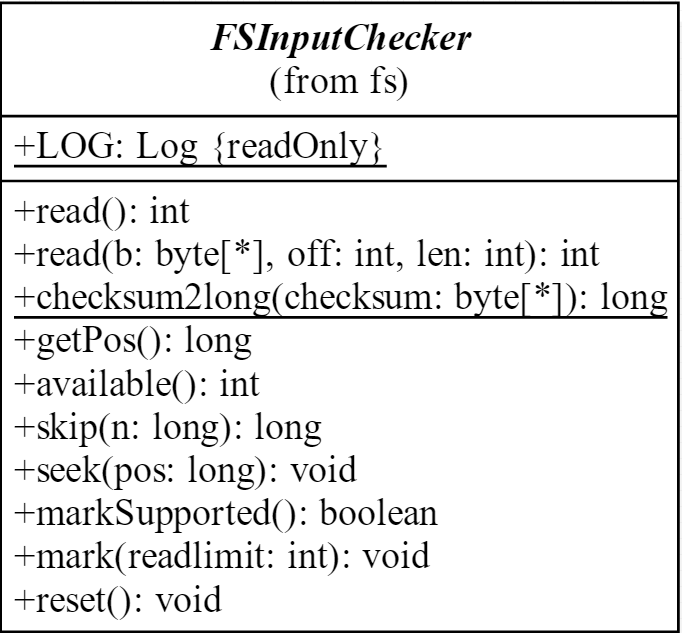
\includegraphics[width=3in,height=3in]{UML/inputstream/FSInputChecker.png}
		\caption{FSInputChecker}
		\label{fig:graph7}
	\end{figure}
	\subsubsection{FilterFileSystem} 
	FilterFileSystem 类包含了一个其它的文件系统的实例 fs,并将其作为基本的文件系统。FilterFileSystem 类几乎将所有重写的方法交给了其内部保存的 fs 来处理。但在交给 fs 处理之前,自己可以做一些处理,以此来实现过滤。
	\begin{figure}
		\centering
		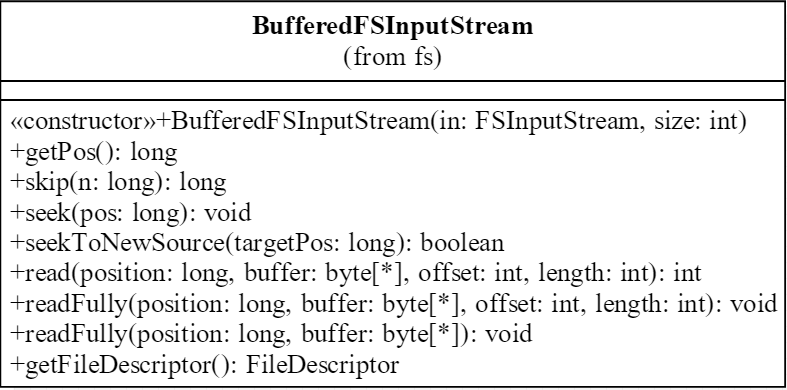
\includegraphics[width=3in,height=3in]{UML/inputstream/BufferedFSInputStream.png}
		\caption{BufferedFSInputStream}
		\label{fig:graph8}
	\end{figure}
	
	\subsubsection{BufferedInputStream} 
	BufferedInputStream 是缓冲输入流。它继承于FilterInputStream。
	BufferedInputStream 的作用是为另一个输入流添加一些功能,例如,提供“缓冲功能”以及支持“mark()标记”和“reset()重置方法”。
	BufferedInputStream 本质上是通过一个内部缓冲区数组实现的。例如,在新建某输入流对应的BufferedInputStream后,当我们通过read()读取输入流的数据时,BufferedInputStream会将该输入流的数据分批的填入到缓冲区中。每当缓冲区中的数据被读完之后,输入流会再次填充数据缓冲区;如此反复,直到我们读完输入流数据位置。
	
	%% end
	\endinput

\subsubsection{DataInput}
\label{sec:uml:input:datainput}

Java 官方的包中提供了一个名叫 \lstinline|DataInput| 的接口,而 Java 官方的文档中有如下描述
\begin{quote}
    The DataInput interface provides for reading bytes from a binary stream and reconstructing from them
    data in any of the Java primitive types. There is also a facility for reconstructing a String from
    data in modified UTF-8 format. 
\end{quote}

大致意思是 \lstinline|DataInput| 提供了一个能将二进制流中的“字节”重新组合成所需要的 Java 基础数据类型的数据。
同时还提供了对 UTF-8 的支持与格式化。其定义了14个\lstinline|read|方法,来提供对基础类型读取和UTF读取的支持。
同时官方的文档中还提供了解析的“标准”。

图 \ref{fig:datainput} 是 这个类的UML类图。
\begin{figure}
\centering
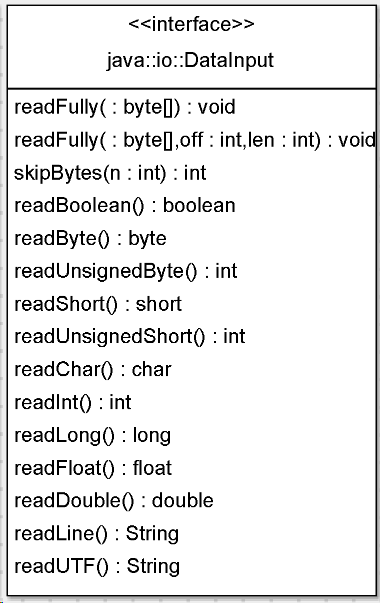
\includegraphics{UML/inputstream/datainput}
\caption{DataInput 接口的 UML 类图}
\label{fig:datainput}
\end{figure}

下面是这个接口的代码。
\begin{java}
interface DataInput {
\end{java}
首先显示两个读取全部字节的方法。
\begin{java}    
    void readFully(byte b[]) throws IOException;
    void readFully(byte b[], int off, int len) throws IOException;
\end{java}
然后是一个用于跳过一定字节数目的方法,或者说是读取不返回。
\begin{java}    
    int skipBytes(int n) throws IOException;
\end{java}
之后是一些用于从中读取Java基础类型的方法,从二进制流进行反序列化。
\begin{java}   
    boolean readBoolean() throws IOException;
    byte readByte() throws IOException;
    int readUnsignedByte() throws IOException;
    short readShort() throws IOException;
    int readUnsignedShort() throws IOException;
    char readChar() throws IOException;
    int readInt() throws IOException;
    long readLong() throws IOException;
    float readFloat() throws IOException;
    double readDouble() throws IOException;
\end{java}
最后是读取一整行或者是读取 UTF 编码内容的内容。
\begin{java}
    String readLine() throws IOException;
    String readUTF() throws IOException;
}
\end{java}


\subsubsection{DataInputStream}
\label{sec:uml:input:datainputstream}

在 Java 官方的 IO 包中,官方提供了 \lstinline|DataInputStream| 这个类。
在 API 文档中的描述如下
\begin{quote}
  A data input stream lets an application read primitive Java data types from an underlying input stream in a machine-independent way. 
  An application uses a data output stream to write data that can later be read by a data input stream.

  DataInputStream is not necessarily safe for multithreaded access. Thread safety is optional and is the responsibility of users of methods in this class.
\end{quote}

这一段描述交代了两件事, \lstinline|DataInputStream| 是一个用于读取“原始”的Java数据,并且与硬件底层无关。第二件事指出了其不是线程安全的,线程安全由用户保证。

\lstinline|DataInputStream| 继承自 \lstinline|FilterInputStream|, 同时实现了 \lstinline|DataInput| 接口。
\lstinline|DataInputStream| 的使用基本上就是以 \lstinline|DataInputStream var = new DataInputStream(new InputStream(..));| 的方式使用,类似与于
\lstinline|BufferedInputStream|。其提供了17个 read 函数的实例,分贝可以读取字节,布尔类型,字符类型,浮点类型, 和整数类型,同是提供了读取一行,和跳过字节的功能。
同时还从 \lstinline|FilterInputStream| 继承了一些其他的方法。

%% 类图
如下图 \ref{fig:datainputstream} 是 这个类的 UML 类图。
\begin{figure}
\centering
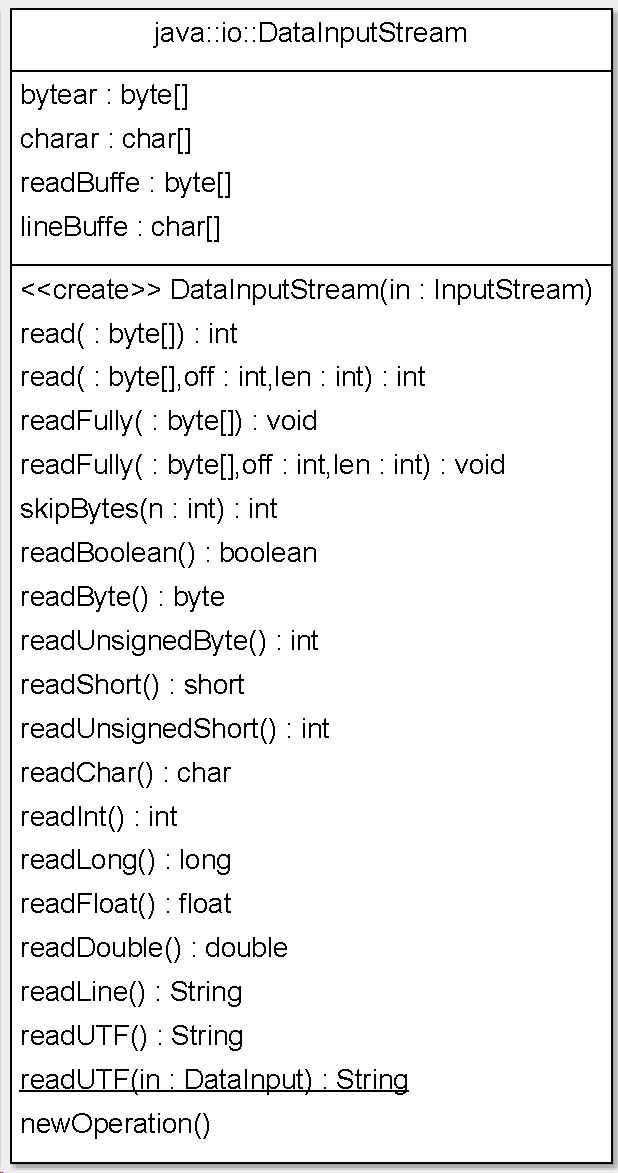
\includegraphics{UML/inputstream/datainputstream}
\caption{DataInputStream 类的 UML 类图}
\label{fig:datainputstream}
\end{figure}

%% 代码(主要的read)
这个类主要继承于\lstinline|FilterInputStream| 并实现了 DataInput 接口。
\begin{java}
public class DataInputStream extends FilterInputStream implements DataInput {
\end{java}
类似的,构造函数也是直接“输入” 一个\lstinline|InputStream|。
\begin{java}
    public DataInputStream(InputStream in) {
        /*...*/
    }    
\end{java}
其提供了许多读取的用的方法。有一些相对比较常见的方法,接受字节输入。 
\begin{java}
    public final int read(byte b[]) throws IOException {
        /*...*/
    }
    
    public final int read(byte b[], int off, int len) throws IOException {
        /*...*/
    }
    
    public final void readFully(byte b[]) throws IOException {
        /*...*/
    }
    
    public final void readFully(byte b[], int off, int len) throws IOException {
        /*...*/
    }
\end{java}
同时还提供了跳过字节的方法,用来跳过特定数目的字节内容。
\begin{java}
    public final int skipBytes(int n) throws IOException {
        /*...*/
    }
\end{java}
此外就是一些用于读取特定数据内容的 “read”方法。
包括读取:布尔类型,字节类型,无符号字节类型,短整型,无符号短整型,字符类型,整型,长整型,单精度浮点,双精度浮点等数据的功能。
\begin{java}    
    public final boolean readBoolean() throws IOException {
        /*...*/
    }
    
    public final byte readByte() throws IOException {
        /*...*/
    }
    
    public final int readUnsignedByte() throws IOException {
        /*...*/
    }
    
    public final short readShort() throws IOException {
        /*...*/
    }
    
    public final int readUnsignedShort() throws IOException {
        /*...*/
    }
    
    public final char readChar() throws IOException {
        /*...*/
    }
    
    public final int readInt() throws IOException {
        /*...*/
    }
    
    public final long readLong() throws IOException {
        /*...*/
    }
    
    public final float readFloat() throws IOException {
        /*...*/
    }
    
    public final double readDouble() throws IOException {
        /*...*/
    }    
\end{java}
当然也提供了读取一行和读取 UTF 字符集字符的功能。
\begin{java}    
    @Deprecated
    public final String readLine() throws IOException {
        /*...*/
    }
    
    public final String readUTF() throws IOException {
        /*...*/
    }   
}
\end{java}


\subsubsection{FSDataInputStream}
\label{sec:uml:input:fsdatainputstream}

\lstinline{FSDataInputStream} 这个类提供了对 \lstinline|java.io| 包中的 \lstinline|DataInputStream| 支持。
\lstinline{FSDataInputStream} 继承自 \lstinline|DataInputStream|,同时实现了 \lstinline|Seekable|, \lstinline|PositionedReadable|, \lstinline|ByteBufferReadable|, \lstinline|CanSetDropBehind|, \lstinline|CanSetReadahead| 等接口,
以提供搜索,随机读取,以字节的缓冲试读取,以及丢弃缓存等功能。

在 Hadoop 官方的 API 文档中,写着这样的一句话:
\begin{quote}
    Utility that wraps a FSInputStream in a DataInputStream and buffers input through a BufferedInputStream.
\end{quote}
意味着 \lstinline|FSDataInputStream| 融合了 \lstinline|DataInputStream| 和 \lstinline|FSInputStream|,同时提供了
\lstinline|BufferedInputStream| 的输入方式。

\lstinline|FSDataInputStream| 提供了一些列的扩展的读取方法与随机跳转的方法。读取的方法中,主要提供了基于 缓冲区的,和缓冲区池的
读取方法。随机读取与跳转提供了寻找跳转与抛弃跳转的功能。
\lstinline|FSDataInputStream| 再加上继承来的函数,其提供了一个对于分布式文件系统带来的输入流的“使用”。

%% 类图

%% 代码
\subsubsection{HasEnhancedByteBufferAccess}
\label{sec:uml:input:hasenhancedbytebufferaccess}

\lstinline|HasEnhancedByteBufferAccess| 这个接口提供了一个加强的 字节型的,缓冲式的读取方式。
一共提供了两个方法 \lstinline|releaseBuffer()| 和 \lstinline|read()|,分别用于释放和取得一个\lstinline|ByteBuffer|.

%% 类图
如下图 \ref{fig:HasEnhancedByteBufferAccess} 是 这个接口的 UML 类图。
\begin{figure}[h]
\centering
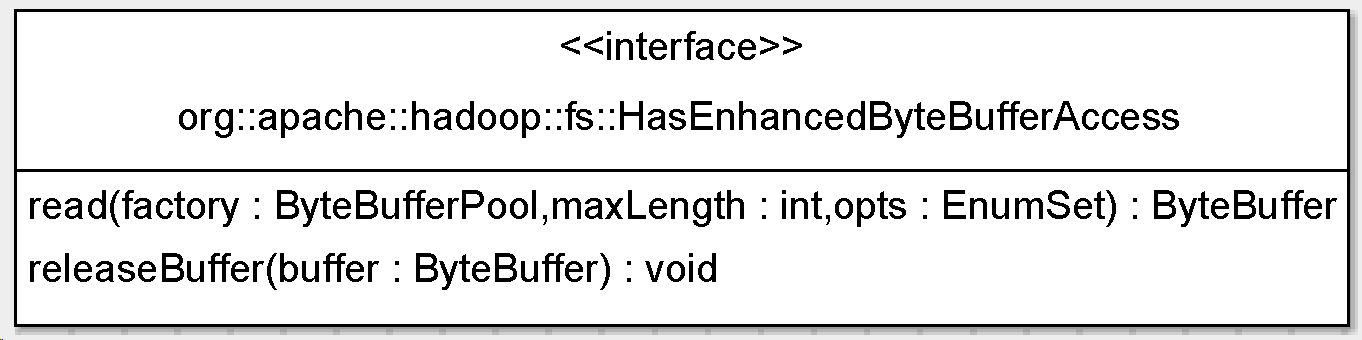
\includegraphics[width=1\linewidth]{HasEnhancedByteBufferAccess}
\caption{HasEnhancedByteBufferAccess 接口的 UML 类图}
\label{fig:HasEnhancedByteBufferAccess}
\end{figure}

%% 代码
这个接口一共定义了两个方法的接口。用于读取一个字节缓冲区,从字节缓冲区池中,同时还有释放的方法。
\begin{java}
@InterfaceAudience.Private
@InterfaceStability.Evolving
public interface HasEnhancedByteBufferAccess {
    public ByteBuffer read(ByteBufferPool factory, int maxLength, EnumSet<ReadOption> opts) throws IOException, UnsupportedOperationException;
    public void releaseBuffer(ByteBuffer buffer);
}    
\end{java}
\endinput
%% outputstream
\section{OutputStream}

\begin{figure}
\centering
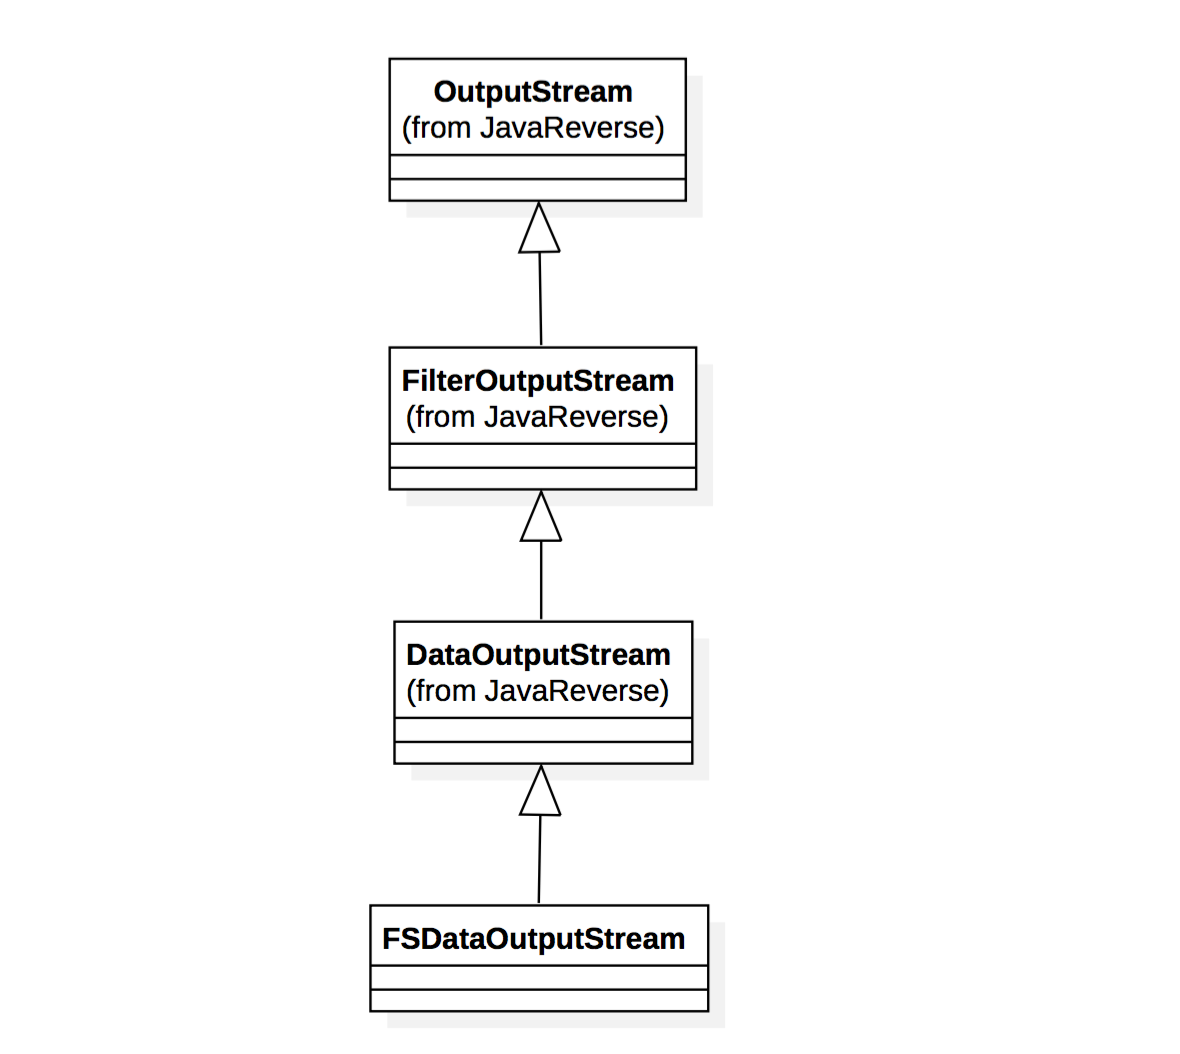
\includegraphics[width =1\linewidth]{11.png}
\caption{outputstream 及其子类}
\label{fig:OutputStream}
\end{figure}


关闭此输出流并释放与此流相关联的任何系统资源。总的来说close 是关闭输出流。封闭流不能执行输出操作,无法重新打开。
该close方法OutputStream不执行任何操作。
\begin{java}
public void close()
\end{java}
刷新此输出流并强制任何缓冲的输出字节被写出。通常来说flush是指出,如果以前写入的任何字节已经通过输出流的实现被缓冲,则这些字节应该立即被写入到它们的预定目的地。
如果此流的预期目标是由底层操作系统(例如文件)提供的抽象,那么刷新流仅保证先前写入流的字节传递到操作系统进行写入; 它并不保证它们实际上被写入物理设备,如磁盘驱动器。

在该flush方法中OutputStream不执行任何操作。
\begin{java}
public void flush()
\end{java}
len将从偏移量开始的指定字节数组的字节写入off此输出流。一般来说write(b, off, len)是数组b中的一些字节按顺序写入输出流; 元素b[off]是写入的第一个字节,b[off+len-1]是此操作写入的最后一个字节。
所述write的方法OutputStream被调用在每个字节中的一个参数的写入方法。鼓励子类覆盖此方法并提供更有效的实现。

如果b是null, NullPointerException则抛出一个。

如果off为负数,或len为负数,或 off+len大于数组的长度 b,则抛出IndexOutOfBoundsException。
\begin{java}
public void write(byte [] b,int off,int len)
\end{java}
将b.length指定字节数组的字节写入此输出流。
\begin{java}
public void write(byte [] b)
\end{java}
将指定的字节写入此输出流。一般来说write是一个字节被写入输出流。要写入的字节是参数的8个低位b。24个高位b被忽略。
子类OutputStream必须为此方法提供一个实现。
\begin{java}
public abstract void write(int b)
\end{java}

FilterOutputStream

创建一个基于指定底层输出流的输出流过滤器。
参数:
out- 要分配给field.out以供以后使用的底层输出流,或者 null如果要创建此实例而不使用底层流。
\begin{java}
public FilterOutputStream(OutputStream  out)
\end{java}
将指定的数据写入byte此输出流。

所述write的方法FilterOutputStream 调用write它的基本输出流的方法,也就是说,它执行out.write(b)中。

实现抽象的写入方法的OutputStream。

\begin{java}
public void write(int b)
\end{java}
将b.length字节写入此输出流。

该write方法FilterOutputStream 调用其write与参数的三个参数的方法b,0和 b.length。

请注意,此方法不 write使用单个参数调用其基础流的单参数方法b。
\begin{java}
public void write(byte [] b)
\end{java}
len从指定的byte数组写入从 偏移量off到该输出流的字节。

所述write的方法FilterOutputStream 调用的write每个一个参数的方法 byte,以输出。

请注意,此方法不会write使用相同的参数调用其底层输入流的方法。子类FilterOutputStream应提供更有效的方法实现。

\begin{java}
public void write(byte [] b,int off,int len)
\end{java}

刷新此输出流,并强制将任何缓冲的输出字节写入流。

所述flush的方法FilterOutputStream 调用flush其基础输出流的方法。
\begin{java}
public void flush()
\end{java}
关闭此输出流并释放与流相关联的任何系统资源。

所述close的方法FilterOutputStream 的调用其flush的方法,然后调用 close它的基本输出流的方法。
\begin{java}
public void close()
\end{java}

DataOutputStream

创建一个新的数据输出流,以将数据写入指定的底层输出流。计数器written设置为零。

\begin{java}
public DataOutputStream(OutputStream  out)
\end{java}
将指定的字节(参数的低8位 b)写入底层输出流。如果没有异常抛出,计数器written将递增 1。

实现write方法OutputStream。
\begin{java}
public void write(int b)
\end{java}
len从指定的字节数组写入字节,从偏移开始off到底层输出流。如果没有异常抛出,计数器written将递增len。
\begin{java}
public void write(byte [] b,int off,int len)
\end{java}
刷新此数据输出流。这将强制任何缓冲的输出字节写入流。

所述flush的方法DataOutputStream 调用flush其基础输出流的方法。
\begin{java}
public void flush()
\end{java}

将boolean底层输出流写入1字节值。该值true作为值写出(byte)1; 该值false将作为值写出(byte)0。如果没有异常抛出,计数器written将递增 1。
\begin{java}
public final void writeBoolean(boolean v)
\end{java}
将byte底层输出流写入1字节值。如果没有异常抛出,计数器 written将递增1。
\begin{java}
public final void writeByte(int v)
\end{java}

将short底层输出流写入两个字节,高字节优先。如果没有异常抛出,计数器 written将递增2。
\begin{java}
public final void writeShort(int v)
\end{java}
将char底层输出流写入2字节值,先将高字节写入。如果没有异常抛出,计数器written将递增2。
\begin{java}
public final void writeChar(int v)
\end{java}
将int底层输出流写入四字节,高位字节。如果没有异常抛出,计数器 written将递增4。
\begin{java}
public final void writeInt(int v)
\end{java}

将long底层输出流写入八字节,高位字节。抛出任何异常,计数器 written增加8。
\begin{java}
public final void writeLong(long v)
\end{java}
将float参数转换为int使用floatToIntBits类中的 方法Float,然后将该int值写入底层输出流,为4字节数量,高字节为首。如果没有异常抛出,计数器written将递增4。

\begin{java}
public final void writeFloat(float v)
\end{java}

将double参数转换为long使用doubleToLongBits类中的 方法Double,然后将该long值作为8字节数量,高字节优先写入底层输出流。如果没有异常抛出,计数器written将递增8。

\begin{java}
public final void writeDouble(double v)
\end{java}

将字符串作为字节序列写入基础输出流。字符串中的每个字符顺序地通过丢弃其高8位来写出。如果没有异常被抛出,计数器written的长度就会增加s。
\begin{java}
public final void writeBytes(String  s)
\end{java}

将字符串写入底层输出流作为一系列字符。每个字符都被写入到数据输出流中,如同通过该writeChar方法一样。如果没有抛出异常,计数器written的长度增加两倍s。
\begin{java}
public final void writeChars(String  s)
\end{java}

使用修改的UTF-8 编码以机器无关方式将字符串写入底层输出流。

首先,将两个字节写入输出流,就像通过writeShort给出要跟随的字节数的 方法一样。该值是实际写出的字节数,而不是字符串的长度。按照长度,字符串的每个字符依次输出,使用修改的UTF-8编码字符。如果没有异常被抛出,计数器 written将增加写入输出流的总字节数。这将至少是两个加上长度str,最多两个加三倍的长度str。


\begin{java}
public final void writeUTF(String str)
\end{java}

返回计数器的当前值,written到目前为止写入此数据输出流的字节数。如果计数器溢出,它将被包装到Integer.MAX\_VALUE。
\begin{java}
public final int size()
\end{java}

FSDataOutputStream

\begin{figure}[h]
\centering
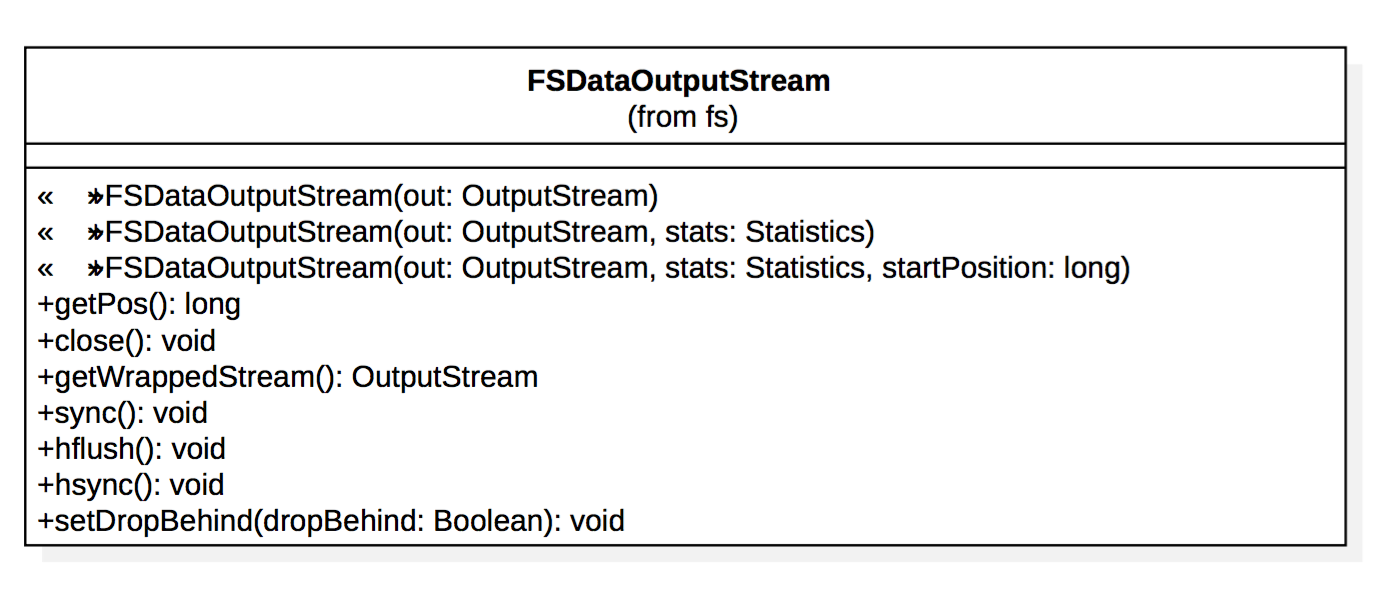
\includegraphics[width =1\linewidth]{1.png}
\caption{FSDataOutputStream}
\label{fig:FSDataOutputStream}
\end{figure}

\begin{figure}[h]
\centering
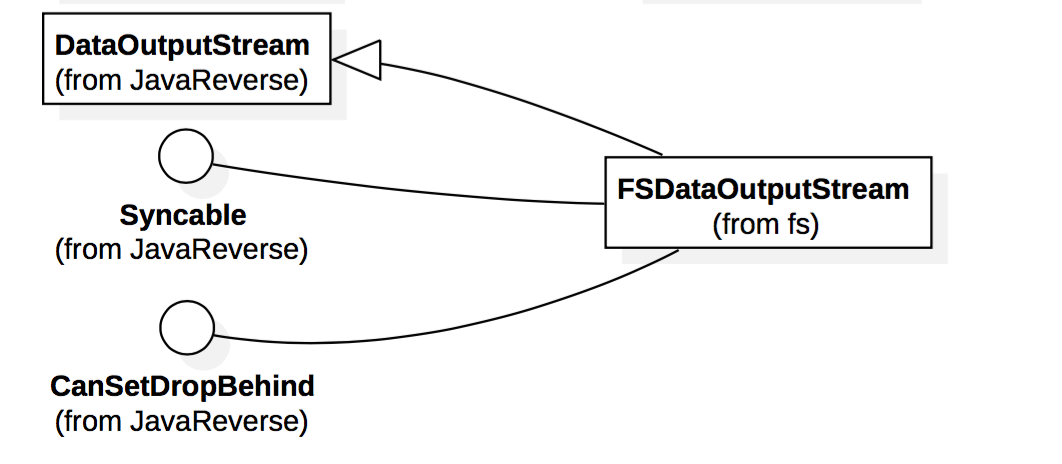
\includegraphics[width =1\linewidth]{2.png}
\caption{Hierarchy of FSDataOutputStream}
\label{fig:Hierarchy of FSDataOutputStream}
\end{figure}

Hadoop 的FileSystem中的create()方法返回了一个FSDataOutputStream对象。与FSDataInputStream一样,它也有一个用于查询位移的方法。但并没有类似于FSDataInputStream中seek()的方法,因为Hadoop不允许向流中的任意位置写数据,我们只能在一个文件的末尾处添加数据。同时2.8.0版本的Hadoop相较于旧版本,多实现了一个接口:CanSetDropBehind。

该接口声明了一个方法:
\begin{java}
public void setDropBehind(Boolean dropBehind) throws IOException
\end{java}
用于判断流是否应该丢弃缓存。

FSDataOutputStream同样实现了getPos()的功能:

\begin{java}
public long getPos() throws IOException
\end{java}
用于获取输入流的当前位置,并返回输入流的当前位置

继承关系:

java.lang.Object -->

java.io.OutputStream -->

java.io.FilterOutputStream -->

java.io.DataOutputStream -->

org.apache.hadoop.fs.FSDataOutputStream



FSDataOutputStream继承自DataOutputStream 并实现了接口Syncable和接口CanSetDropBehind,下面是对该类的具体说明:

三个构造函数:

该构造函数已过时
\begin{java}
@Deprecated
public FSDataOutputStream(OutputStream out) throws IOException {
	this(out, null);
}
\end{java}
该构造函数的参数包括:OutputStream类型的参数,Statistics类的参数
\begin{java}
public FSDataOutputStream(OutputStream out, FileSystem.Statistics stats)throws IOException {
	this(out, stats, 0);
}
\end{java}
该构造函数的参数包括:OutputStream类型的参数,Statistics类的参数和当前流的开始位置。
\begin{java}
public FSDataOutputStream(OutputStream out, FileSystem.Statistics stats,
		     long startPosition) throws IOException {
	super(new PositionCache(out, stats, startPosition));
	wrappedStream = out;
}
\end{java}
获取输入流的当前位置,并返回输入流的当前位置
\begin{java}
public long getPos() throws IOException {
	return position;
}

public long getPos() throws IOException {
	return ((PositionCache)out).getPos();
}
\end{java}
关闭基础输入流
\begin{java}
public void close() throws IOException {
	out.close();
}
\end{java}
刷新客户端中用户缓冲区的数据。在此调用的返回之后,新的读者将看到数据。来自于接口:Syncable
\begin{java}
public void hflush() throws IOException {
	if (wrappedStream instanceof Syncable) {
		((Syncable)wrappedStream).hflush();
    	} else {
      		wrappedStream.flush();
    }
}
\end{java}
将客户端用户缓冲区中的数据一直刷新到磁盘设备(但磁盘可能在其缓存中)。来自于接口:Syncable

\begin{java}
public void hsync() throws IOException {
	if (wrappedStream instanceof Syncable) {
      ((Syncable)wrappedStream).hsync();
	    } else {
      		wrappedStream.flush();
	}
}
\end{java}
配置判断流是否应该丢弃缓存。

参数:dropBehind:判断是否删除缓存

\begin{java}
public void setDropBehind(Boolean dropBehind) throws IOException {
	 try {
	    ((CanSetDropBehind)wrappedStream).setDropBehind(dropBehind);
	  } catch (ClassCastException e) {
	    throw new UnsupportedOperationException("the wrapped stream does " +
	        "not support setting the drop-behind caching setting.");
	  }
	}
\end{java}


\begin{figure}[h]
\centering
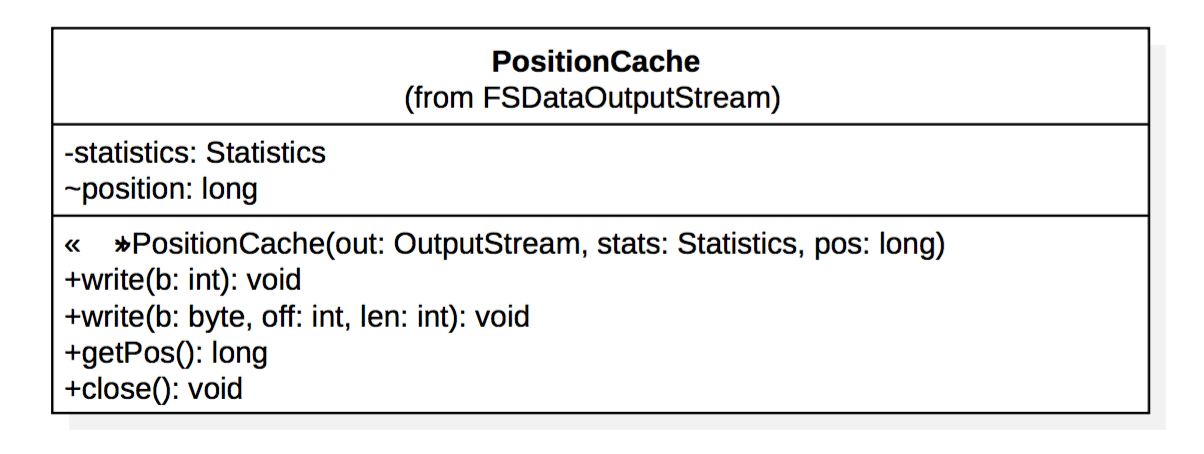
\includegraphics[width =1\linewidth]{3.png}
\caption{PositionCache}
\label{fig:PositionCache}
\end{figure}

FSDataOutputStream 中有一个内部类 PositionCache,其从 FilterOutputStream 派生,提供了缓
存文件指针 position 的功能,并且有一个 statistics 属性,用来统计。


接口:Syncable


\begin{java}
@InterfaceAudience.Public
@InterfaceStability.Evolving
public interface Syncable {
	 @Deprecated
	 public void sync() throws IOException;

	 public void hflush() throws IOException;

	 public void hsync() throws IOException;
}
\end{java}
接口:	CanSetDropBehind
\begin{java}
@InterfaceAudience.Public
@InterfaceStability.Evolving
public interface CanSetDropBehind {
	public void setDropBehind(Boolean dropCache)
	throws IOException, UnsupportedOperationException;
}
\end{java}
HDFS写文件过程
\begin{figure}
\centering
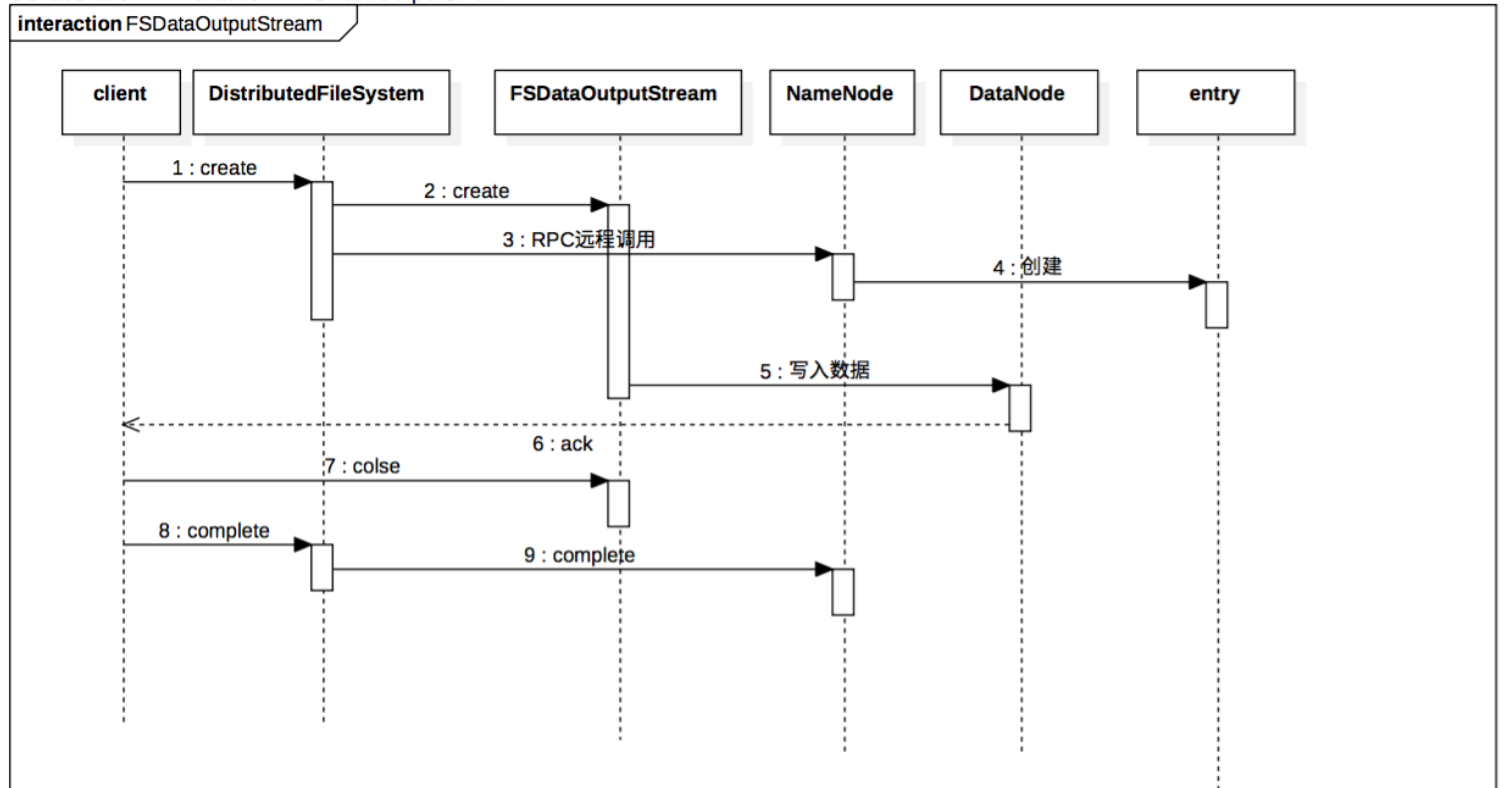
\includegraphics[width =1\linewidth]{write.png}
\caption{HDFS写文件时序图}
\label{fig:HDFS写文件时序图}
\end{figure}

Path

\begin{figure}
\centering
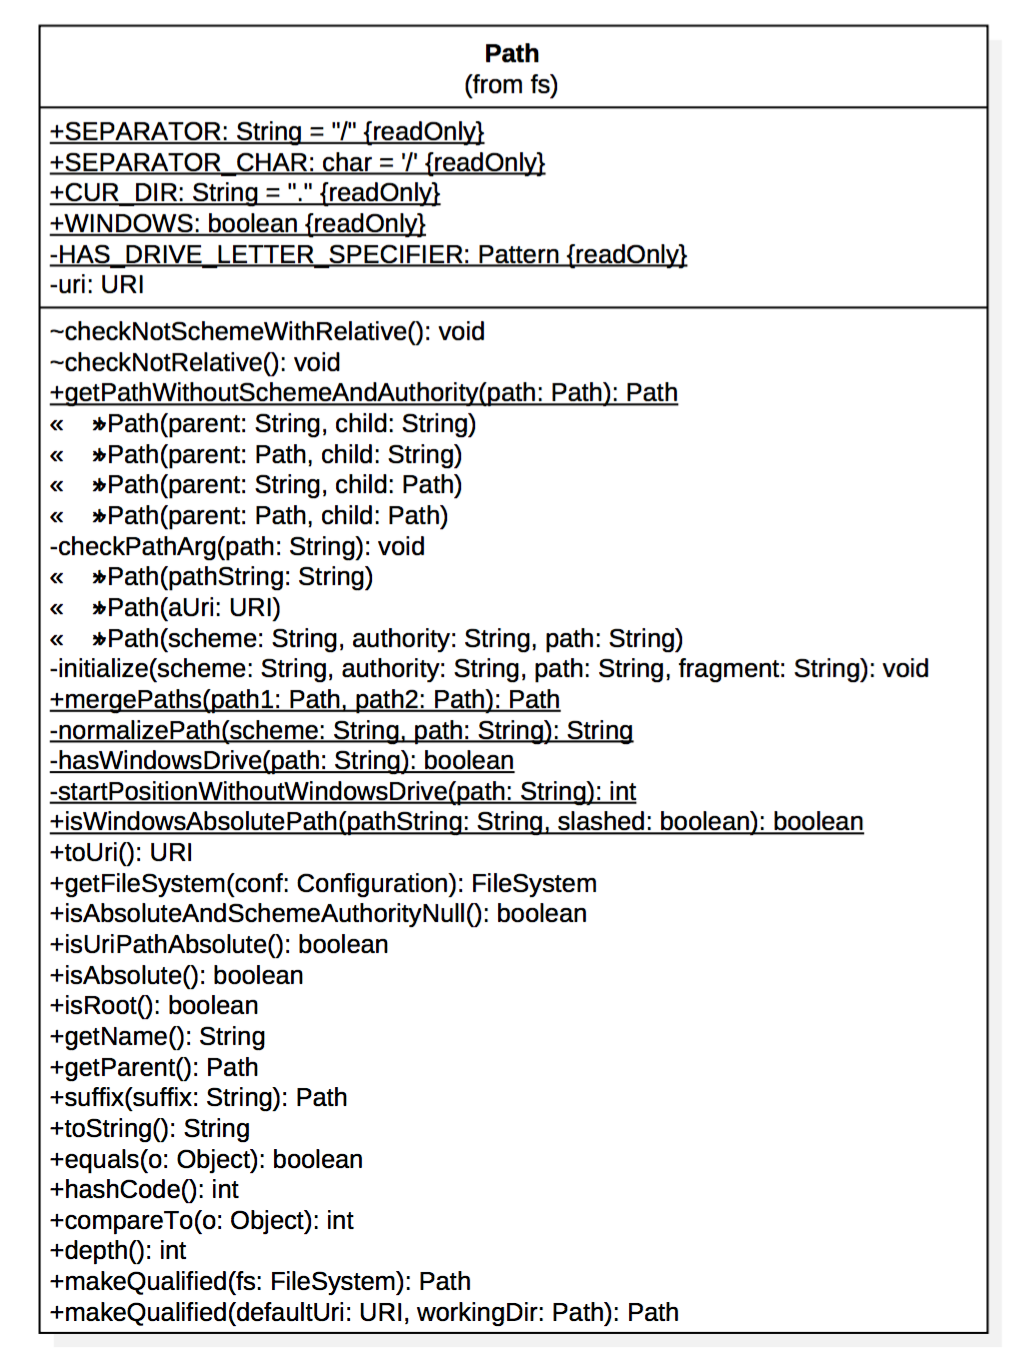
\includegraphics[width =1\linewidth]{6.png}
\caption{Path}
\label{fig:Path}
\end{figure}

\begin{figure}[h]
\centering
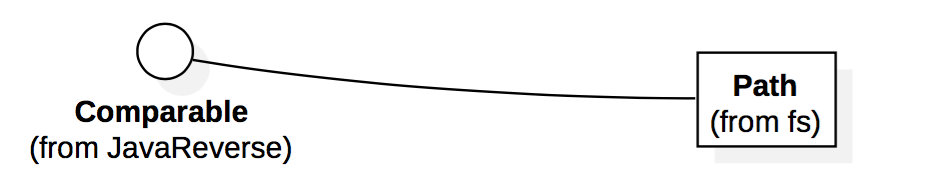
\includegraphics[width =1\linewidth]{7.png}
\caption{Hierarchy of Path}
\label{fig:Hierarchy of Path}
\end{figure}

在一个FileSystem中命名一个文件或目录。路径字符串使用斜杠作为目录分隔符。

Path 对路径进行解析,将参数转换为标准的URI格式,对Path的参数作判断,标准化,字符化等操作。
继承关系:

java.lang.Object -->

org.apache.hadoop.fs.Path


构造函数

基于根据父路径解析的子路径创建新路径。
\begin{java}
public Path(String parent, String child) {
	this(new Path(parent), new Path(child));
}
\end{java}
基于根据父路径解析的子路径创建新路径。
\begin{java}
public Path(Path parent, String child) {
	this(parent, new Path(child));
}
\end{java}
基于根据父路径解析的子路径创建新路径。
\begin{java}
public Path(String parent, Path child) {
	this(new Path(parent), child);
}
\end{java}
基于根据父路径解析的子路径创建新路径。
\begin{java}
public Path(Path parent, Path child) {
	  URI parentUri = parent.uri;
	  String parentPath = parentUri.getPath();
	  if (!(parentPath.equals("/") || parentPath.isEmpty())) {
	    try {
	      parentUri = new URI(parentUri.getScheme(), parentUri.getAuthority(),
	                    parentUri.getPath()+"/", null, parentUri.getFragment());
	    } catch (URISyntaxException e) {
	      throw new IllegalArgumentException(e);
	    }
	  }
	  URI resolved = parentUri.resolve(child.uri);
	  initialize(resolved.getScheme(), resolved.getAuthority(),
	             resolved.getPath(), resolved.getFragment());
	}
\end{java}
从组件构造路径。
\begin{java}
public Path(String scheme, String authority, String path) {
  checkPathArg( path );

  if (hasWindowsDrive(path) && path.charAt(0) != '/') {
    path = "/" + path;
  }

	if (!WINDOWS && path.charAt(0) != '/') {
    path = "./" + path;
  }

  initialize(scheme, authority, path, null);
}
\end{java}
\begin{java}
public int compareTo(Object o) {
  Path that = (Path)o;
  return this.uri.compareTo(that.uri);
}
\end{java}
返回此路径中的元素数。
\begin{java}
public int depth() {
  String path = uri.getPath();
  int depth = 0;
  int slash = path.length()==1 && path.charAt(0)=='/' ? -1 : 0;
  while (slash != -1) {
    depth++;
    slash = path.indexOf(SEPARATOR, slash+1);
	}
	return depth;
}
\end{java}
返回拥有此路径的文件系统。
\begin{java}
public FileSystem getFileSystem(Configuration conf) throws IOException {
  return FileSystem.get(this.toUri(), conf);
}
\end{java}
返回此路径的最终组件。
\begin{java}
public String getName() {
  String path = uri.getPath();
  int slash = path.lastIndexOf(SEPARATOR);
  return path.substring(slash+1);
}
\end{java}
返回路径的父亲, 如果为根, 则为 null。
\begin{java}
public Path getParent() {
  String path = uri.getPath();
  int lastSlash = path.lastIndexOf('/');
  int start = startPositionWithoutWindowsDrive(path);
  if ((path.length() == start) ||               // empty path
      (lastSlash == start && path.length() == start+1)) { // at root
    return null;
  }
	String parent;
  if (lastSlash==-1) {
    parent = CUR_DIR;
  } else {
    parent = path.substring(0, lastSlash==start?start+1:lastSlash);
  }
  return new Path(uri.getScheme(), uri.getAuthority(), parent);
}
\end{java}
返回给定路径的版本, 而不提供方案信息。
\begin{java}
public static Path getPathWithoutSchemeAndAuthority(Path path) {
  Path newPath = path.isUriPathAbsolute() ?
    new Path(null, null, path.toUri().getPath()) :
    path;
  return newPath;
}
\end{java}
返回路径组件
\begin{java}
public boolean isAbsolute() {
   return isUriPathAbsolute();
}
\end{java}
\begin{java}
public boolean isAbsoluteAndSchemeAuthorityNull() {
  return  (isUriPathAbsolute() &&
      uri.getScheme() == null && uri.getAuthority() == null);
}
\end{java}
\begin{java}
public boolean isUriPathAbsolute() {
  int start = startPositionWithoutWindowsDrive(uri.getPath());
  return uri.getPath().startsWith(SEPARATOR, start);
}
\end{java}

如果且仅当此路径表示文件系统的根, 则返回 true。
\begin{java}
public boolean isRoot() {
  return getParent() == null;
}
\end{java}
确定给定的路径字符串是否表示 windows 上的绝对路径。
\begin{java}
public static boolean isWindowsAbsolutePath(final String pathString,
                                            final boolean slashed) {
  int start = startPositionWithoutWindowsDrive(pathString);
  return start > 0
      && pathString.length() > start
      && ((pathString.charAt(start) == SEPARATOR_CHAR) ||
          (pathString.charAt(start) == '\\'));
}
\end{java}
\begin{java}
public Path makeQualified(URI defaultUri, Path workingDir ) {
  Path path = this;
  if (!isAbsolute()) {
    path = new Path(workingDir, this);
  }

  URI pathUri = path.toUri();

  String scheme = pathUri.getScheme();
  String authority = pathUri.getAuthority();
  String fragment = pathUri.getFragment();

  if (scheme != null &&
      (authority != null || defaultUri.getAuthority() == null))
    return path;
  if (scheme == null) {
    scheme = defaultUri.getScheme();
  }

  if (authority == null) {
    authority = defaultUri.getAuthority();
    if (authority == null) {
      authority = "";
    }
  }
  URI newUri = null;
  try {
    newUri = new URI(scheme, authority ,
      normalizePath(scheme, pathUri.getPath()), null, fragment);
  } catch (URISyntaxException e) {
    throw new IllegalArgumentException(e);
  }
  return new Path(newUri);
}
\end{java}
合并两路径, 使第二个路径相对于第一个路径被追加
\begin{java}
public static Path mergePaths(Path path1, Path path2) {
  String path2Str = path2.toUri().getPath();
  path2Str = path2Str.substring(startPositionWithoutWindowsDrive(path2Str));
  return new Path(path1.toUri().getScheme(),
      path1.toUri().getAuthority(),
      path1.toUri().getPath() + path2Str);
}
在路径中的最终名称中添加一个后缀。
\begin{java}
public Path suffix(String suffix) {
  return new Path(getParent(), getName()+suffix);
}
\end{java}
将此路径转换为 uri。
\begin{java}
public URI toUri() { return uri; }
\end{java}

QuotaUsage

\begin{figure}[h]
\centering
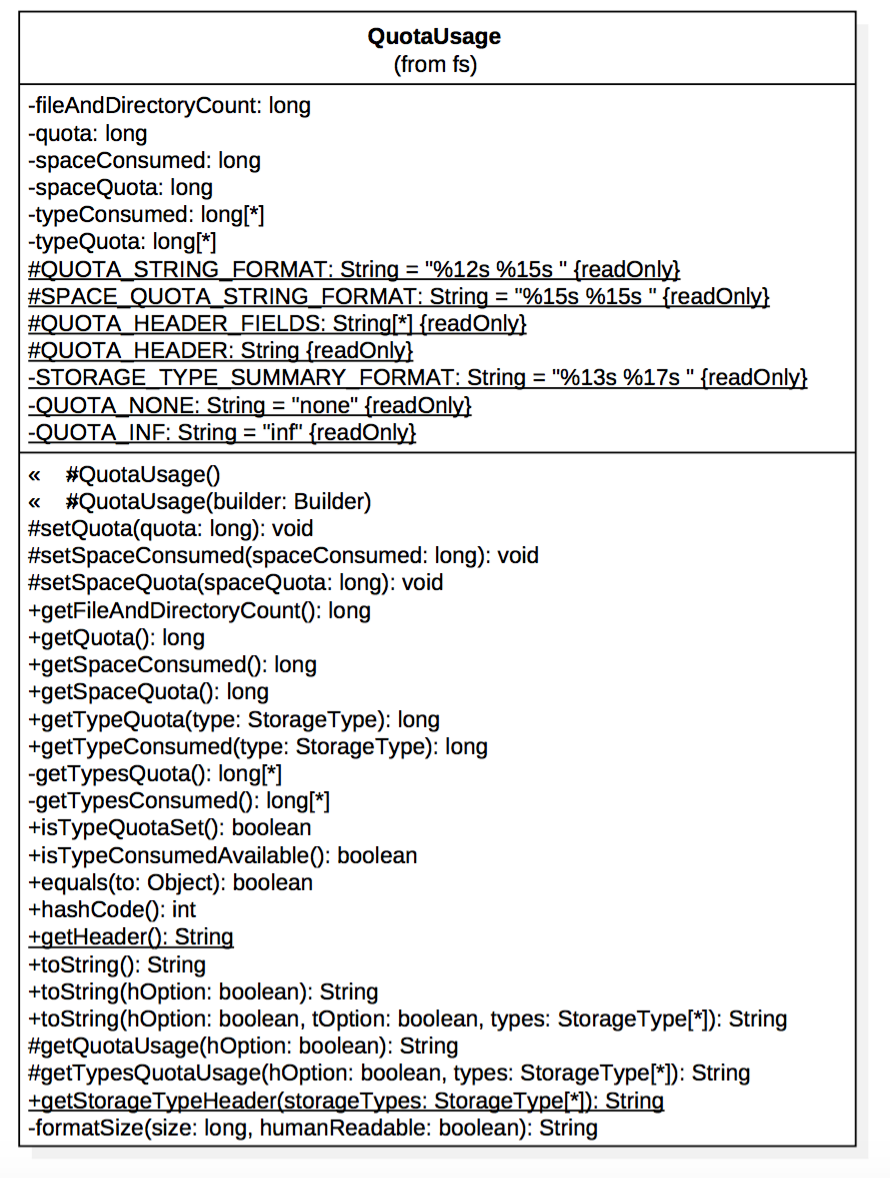
\includegraphics[width =1\linewidth]{8.png}
\caption{QuotaUsage}
\label{fig:QuotaUsage}
\end{figure}

存储目录的配额分配情况。

Quota有以下三种:

Name Quotas : 限制某个目录下的文件和文件夹数量

Space Quotas : 设置某个目录的空间大小

Type Quotas : 设置某个目录的类型数量

fileAndDirectoryCount:文件和目录数量

quota:命名空间的quota(限制文件数)

spaceQuota:物理空间的quota (限制磁盘空间占用大小)

spaceConsumed:消耗的物理空间

typeQuota:类型的quota(限制类型数)

typeConsumed:消耗的类型数

返回输出的标头。
\begin{java}
public static String getHeader() {
  return QUOTA_HEADER;
}
\end{java}
返回目录配额
\begin{java}
public long getQuota() {
  return quota;
}
\end{java}
返回已消耗的(磁盘)空间
\begin{java}
public long getSpaceConsumed() {
  return spaceConsumed;
}
\end{java}
返回 (磁盘) 空间配额。
\begin{java}
public long getSpaceQuota() {
  return spaceQuota;
}
\end{java}
返回 StorageTypes 的标题。
\begin{java}
public static String getStorageTypeHeader(List<StorageType> storageTypes) {
  StringBuffer header = new StringBuffer();

  for (StorageType st : storageTypes) {
    String storageName = st.toString();
    header.append(String.format(STORAGE_TYPE_SUMMARY_FORMAT,
        storageName + "_QUOTA", "REM_" + storageName + "_QUOTA"));
  }
  return header.toString();
}
\end{java}
返回消耗的存储类型。
\begin{java}
public long getTypeConsumed(StorageType type) {
  return (typeConsumed != null) ? typeConsumed[type.ordinal()] : 0;
}
\end{java}
返回消耗的类型配额
\begin{java}
public long getTypeQuota(StorageType type) {
  return (typeQuota != null) ? typeQuota[type.ordinal()] : -1;
}
\end{java}
如果有任何存储类型的消耗信息可用, 则返回 true。
\begin{java}
public boolean isTypeConsumedAvailable() {
  if (typeConsumed == null) {
    return false;
  }
  for (StorageType t : StorageType.getTypesSupportingQuota()) {
    if (typeConsumed[t.ordinal()] > 0) {
      return true;
    }
  }
  return false;
}
\end{java}
如果有任何存储类型配额已被设置, 则返回 true。
\begin{java}
public boolean isTypeQuotaSet() {
  if (typeQuota == null) {
    return false;
  }
  for (StorageType t : StorageType.getTypesSupportingQuota()) {
    if (typeQuota[t.ordinal()] > 0) {
      return true;
    }
  }
  return false;
}
\end{java}

ContentSummary

\begin{figure}[h]
\centering
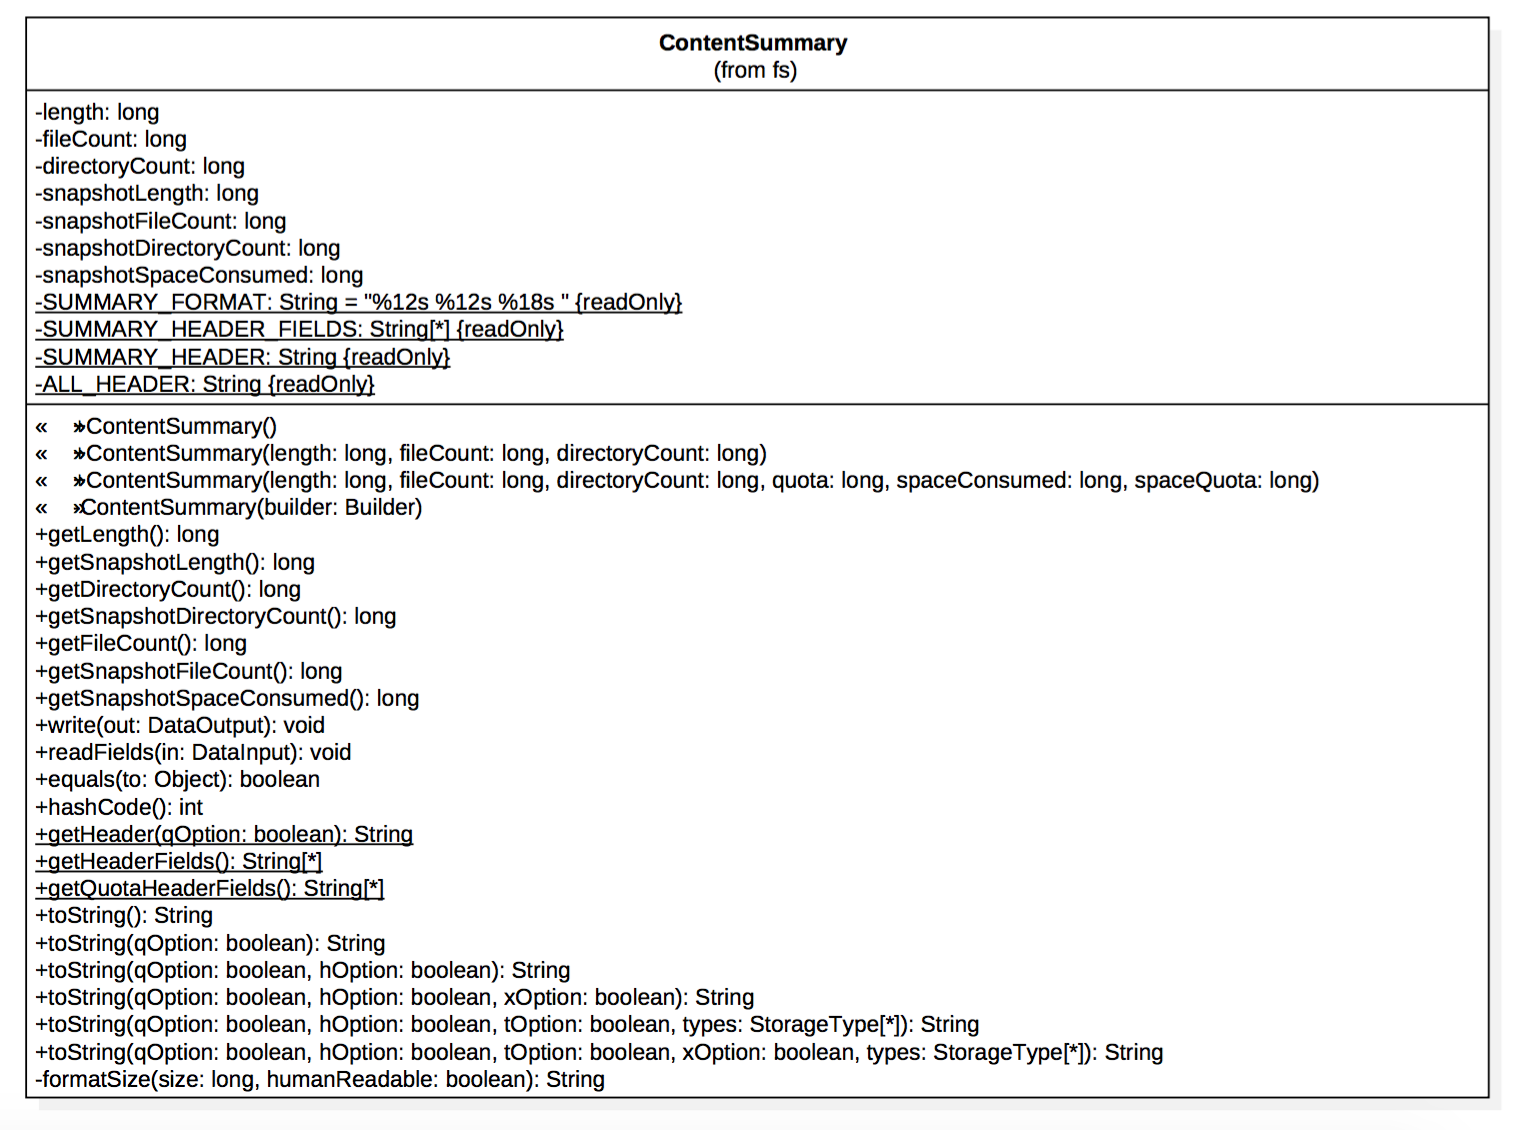
\includegraphics[width =1\linewidth]{9.png}
\caption{ContentSummary}
\label{fig:ContentSummary}
\end{figure}

\begin{figure}[h]
\centering
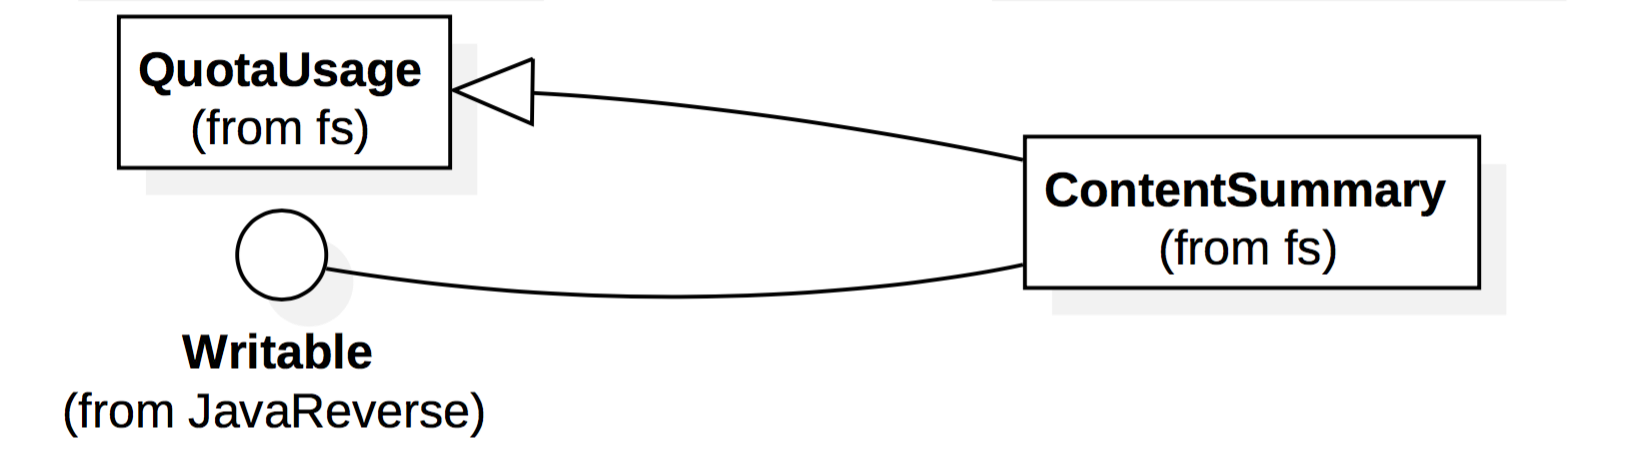
\includegraphics[width =1\linewidth]{10.png}
\caption{Hierarchy of ContentSummary}
\label{fig:Hierarchy of ContentSummary}
\end{figure}

ContentSummary 存储内容(目录或文件)的摘要。

类存储有关文件或目录的一些信息,包括文件长度,文件数量,目录数量,
磁盘配额,已用空间大小,剩余空间大小。

构造函数
\begin{java}
private ContentSummary(Builder builder) {
  super(builder);
  this.length = builder.length;
  this.fileCount = builder.fileCount;
  this.directoryCount = builder.directoryCount;
  this.snapshotLength = builder.snapshotLength;
  this.snapshotFileCount = builder.snapshotFileCount;
  this.snapshotDirectoryCount = builder.snapshotDirectoryCount;
  this.snapshotSpaceConsumed = builder.snapshotSpaceConsumed;
}
\end{java}
返回输出的标题。如果qOption为false,输出目录数,文件数和内容大小; 如果qOption为真,则输出配额和剩余配额
\begin{java}
public static String getHeader(boolean qOption) {
  return qOption ? ALL_HEADER : SUMMARY_HEADER;
}
\end{java}
从摘要标题返回字段的名称。
\begin{java}
public static String[] getHeaderFields() {
  return SUMMARY_HEADER_FIELDS;
}
\end{java}
返回配额摘要中使用的字段的名称。
\begin{java}
public static String[] getQuotaHeaderFields() {
  return QUOTA_HEADER_FIELDS;
}
\end{java}
以输出格式返回对象的字符串表示形式。如果qOption为false,输出目录数,文件数和内容大小; 如果qOption为真,则输出配额和剩余配额。
\begin{java}
public String toString(boolean qOption) {
  return toString(qOption, false);
}
\end{java}
以输出格式返回对象的字符串表示形式。

参数:

qOption - 指示是否需要打印配额的标志

hOption - 一个标志,指示是否使用可读的输出


返回:
对象的字符串表示形式
\begin{java}
public String toString(boolean qOption, boolean hOption) {
  return toString(qOption, hOption, false, null);
}
\end{java}
以输出格式返回对象的字符串表示形式。

参数:

qOption - 指示是否需要打印配额的标志

hOption - 指示是否使用人类可读输出的标志

xOption - 一个标志,指示从快照计算是否包括在输出中

返回:

对象的字符串表示形
\begin{java}
public String toString(boolean qOption, boolean hOption, boolean xOption) {
  return toString(qOption, hOption, false, xOption, null);
}
\end{java}
以输出格式返回对象的字符串表示形式。

参数:

qOption - 指示是否需要打印配额的标志

hOption - 一个标志,指示是否使用可读的输出

tOption - 表示存储类型是否显示配额的标志

types - 要显示的存储类型

返回:

对象的字符串表示形式

\begin{java}
public String toString(boolean qOption, boolean hOption,
                       boolean tOption, List<StorageType> types) {
  return toString(qOption, hOption, tOption, false, types);
}
\end{java}
以输出格式返回对象的字符串表示形式。

如果qOption为false,输出目录数,文件数和内容大小; 如果qOption为真,则输出配额和剩余配额。如果hOption为false,如果hOption为true,则以字节为单位返回文件大小,如果tOption为true,则文件大小返回为人类可读取,如果tOption为false,则显示存储类型的配额,与toString(boolean,boolean)相同的逻辑if xOption为false,如果xOption为真,则输出包括从快照计算,输出不包括快照中的计算。

参数:

qOption - 指示是否需要打印配额的标志

hOption - 指示是否使用人类可读输出的标志

tOption - 表示存储类型是否显示配额的标志

xOption - 一个标志,指示从快照计算是否包括在输出中

types - 要显示的存储类型

返回:

对象的字符串表示形式

\begin{java}
public String toString(boolean qOption, boolean hOption, boolean tOption,
    boolean xOption, List<StorageType> types) {
  String prefix = "";
  if (tOption) {
    return getTypesQuotaUsage(hOption, types);
  }

  if (qOption) {
    prefix = getQuotaUsage(hOption);
  }

  if (xOption) {
    return prefix + String.format(SUMMARY_FORMAT,
        formatSize(directoryCount - snapshotDirectoryCount, hOption),
        formatSize(fileCount - snapshotFileCount, hOption),
        formatSize(length - snapshotLength, hOption));
  } else {
    return prefix + String.format(SUMMARY_FORMAT,
        formatSize(directoryCount, hOption),
        formatSize(fileCount, hOption),
        formatSize(length, hOption));
  }
}
\end{java}
FSOutputSummer
\begin{figure}[h]
\centering
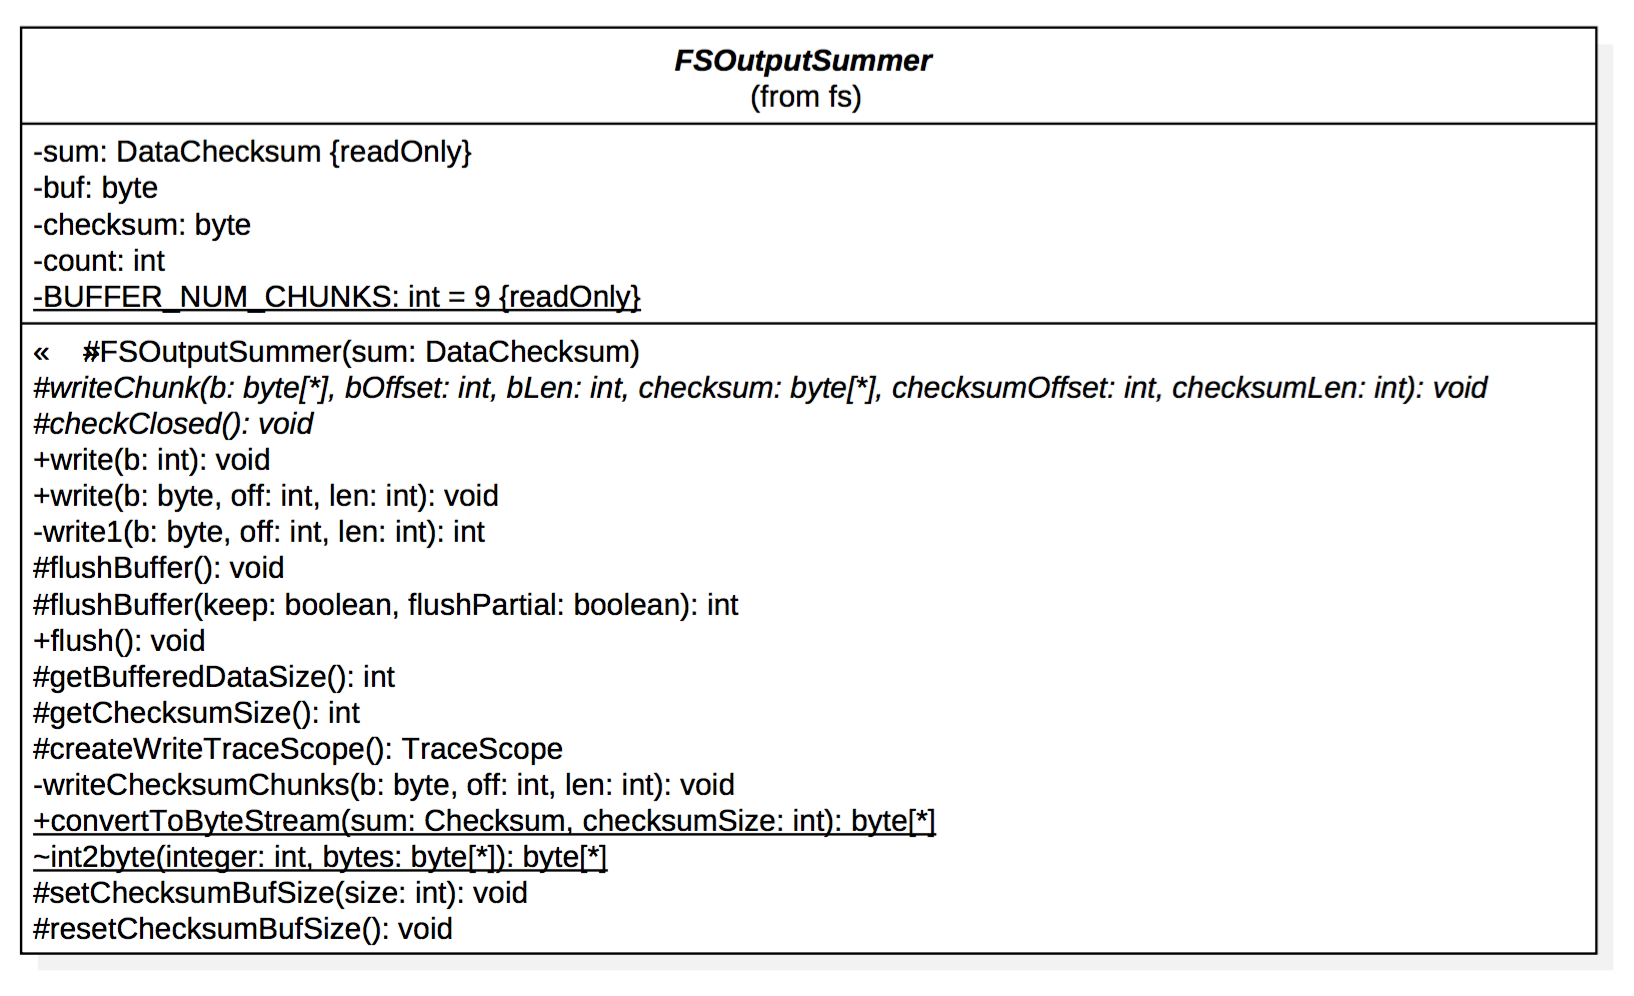
\includegraphics[width =1\linewidth]{4.png}
\caption{FSOutputSummer}
\label{fig:FSOutputSummer}
\end{figure}

\begin{figure}[h]
\centering
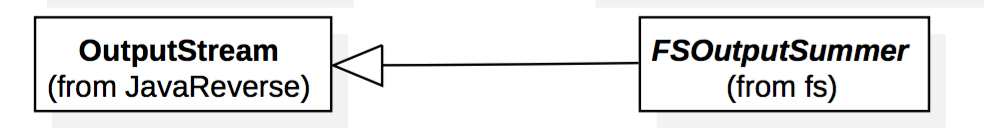
\includegraphics[width =1\linewidth]{5.png}
\caption{Hierarchy of FSOutputSummer}
\label{fig:Hierarchy of FSOutputSummer}
\end{figure}

构造函数:
\begin{java}
protected FSOutputSummer(DataChecksum sum) {
  this.sum = sum;
  this.buf = new byte[sum.getBytesPerChecksum() * BUFFER_NUM_CHUNKS];
  this.checksum = new byte[getChecksumSize() * BUFFER_NUM_CHUNKS];
  this.count = 0;
}
\end{java}

\endinput

%% filesystem
\section{FileSystem}
    \begin{figure}[h]
        \centering
        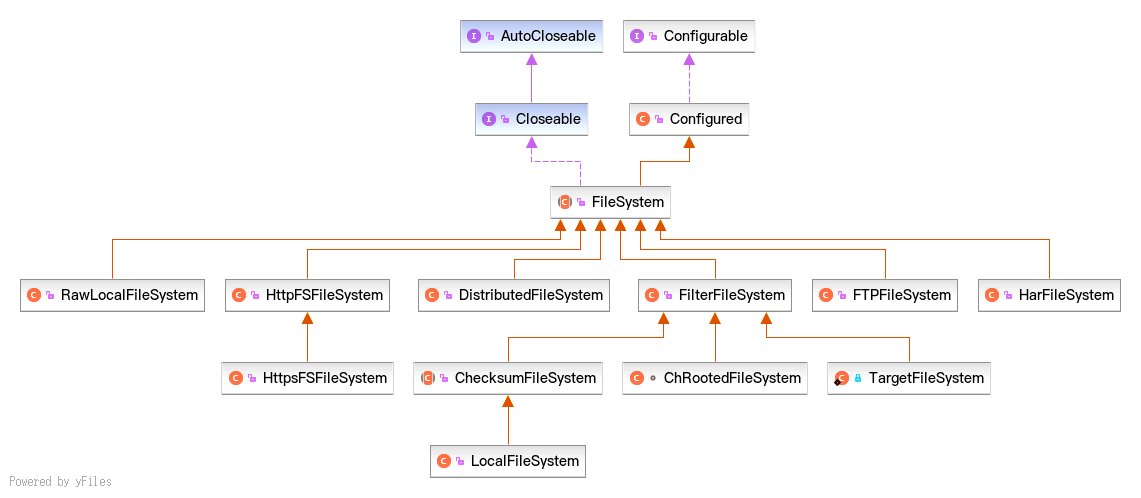
\includegraphics[width=1\linewidth]{filesystemclass}
        \caption{FileSystem 类的 UML 类图}
        \label{fig:filesystemclass}
    \end{figure}
\subsection{}
    \textit{FileSystem}作为文件系统最顶层抽象类,描述了一个文件系统的\textbf{抽象定义},继承了\textit{org.apache.hadoop.conf.Configured}配置基类,并实现了\textit{java.io.Closeable}接口。提供了从XML配置文件生成符合配置描述的文件系统的功能。\\
    \textit{FileSystem}抽象类定义了文件系统所具有的\textbf{基本特征}和\textbf{基本操作}。\textit{FileSystem}具有以下属性:
    \begin{java}[caption=FileSystem attribute]
public static final String FS_DEFAULT_NAME_KEY = 
    CommonConfigurationKeys.FS_DEFAULT_NAME_KEY;
public static final String DEFAULT_FS = 
    CommonConfigurationKeys.FS_DEFAULT_NAME_DEFAULT;

public static final Log LOG = LogFactory.getLog(FileSystem.class);

public static final int SHUTDOWN_HOOK_PRIORITY = 10;

public static final String TRASH_PREFIX = ".Trash";

static final Cache CACHE = new Cache();

private Cache.Key key;

private static final Map<Class<? extends FileSystem>, Statistics> 
    statisticsTable =
        new IdentityHashMap<Class<? extends FileSystem>, Statistics>();

protected Statistics statistics;

private Set<Path> deleteOnExit = new TreeSet<Path>();

    \end{java}
    其中\textit{Cache CACHE}用于缓存已打开的,可缓存的文件系统,启用Cache可以直接\textbf{复用}已打开的文件系统而不必每次都从配置文件生成新的文件系统实例。\\
    \textit{Cache.Key key}所包含的内容就是一个URI的信息及其用户名,作为\textit{Cache}中\textit{Map}的键,与\textit{Cache}一同提供了通过一个合法的URI信息与用户名快速获取到缓存中存在的一个文件系统的对象,从而能够获取到指定文件系统中文件信息的功能。\\
    \textit{statisticsTable} 主要用于保存文件系统的统计信息,作为其\textit{Value}的\textit{Statistics}类使用了\textit{java.util.concurrent.atomic}包中的\textbf{原子变量}属性,提高统计信息的\textbf{一致性},保证\textbf{线程安全}的原子读写操作的同时,提高了\textbf{并行性能}。\\
        \textit{deleteOnExit}作为文件缓存,用来收集当前缓存中的文件\textit{Path}。当文件系统关闭或JVM退出的时候,调用同步方法\textit{processDeleteOnExit}将缓存中的文件全部安全删除。\\
    \\
    \textit{FileSystem}为用户提供了一个访问不同文件系统的统一的\textbf{接口},屏蔽了不同文件系统操作访问上的\textbf{差异性}。其主要提供的方法可以分为两大类:一部分是处理文件和目录相关的事务,另一部分则是文件的读写操作。\\
    以下是\textit{FileSystem}中定义的12个抽象方法,这12个方法应该是一个文件系统应具有的\textbf{基本操作},可归纳为获取文件系统URI,打开文件,创建文件,追加文件,重命名文件,删除文件,获取文件列表,获取和设置工作目录,创建文件夹,获取文件状态。其具体的实现则是取决于不同的文件系统的特点。
    \begin{java}[caption=FileSystem abstract method]
public abstract URI getUri();

public abstract FSDataInputStream open(Path f, int bufferSize) throws IOException;

public abstract FSDataOutputStream create(Path f,
    FsPermission permission,
    boolean overwrite,
    int bufferSize,
    short replication,
    long blockSize,
    Progressable progress) throws IOException;

public abstract FSDataOutputStream append(Path f, int bufferSize, Progressable progress) throws IOException;

public abstract boolean rename(Path src, Path dst) throws IOException;

public abstract boolean delete(Path f) throws IOException;

public abstract boolean delete(Path f, boolean recursive) throws IOException;

public abstract FileStatus[] listStatus(Path f) throws IOException;

public abstract void setWorkingDirectory(Path new_dir);

public abstract Path getWorkingDirectory();

public abstract boolean mkdirs(Path f, FsPermission permission) throws IOException;

public abstract FileStatus getFileStatus(Path f) throws IOException;

    \end{java}

\subsection{基于FileSystem实现的文件系统概述}
    \subsubsection{RawLocalFileSystem}
        \textit{RawLocalFileSystem}是\textit{Hadoop}中实现的本地文件系统,在该类中与文件元数据和目录相关的操作,都是通过\textbf{装饰器模式}适配到\textit{java.io.File}的对应API来完成的。\\
        \textit{LocalFSFileInputStream}的构造函数如下:
        \begin{java}[caption=LocalFSFileInputStream]
class LocalFSFileInputStream extends FSInputStream {
    public LocalFSFileInputStream(Path f) throws IOException {
        this.fis = new TrackingFileInputStream(pathToFile(f));
    }
}
        \end{java}
        \begin{java}[caption=TrackingFileInputStream]
class TrackingFileInputStream extends FileInputStream {
    public TrackingFileInputStream(File f) throws IOException {
        super(f);
    }
}
        \end{java}
    可以看出,\textit{LocalFSFileInputStream}中包装了\textit{TrackingFileInputStream},而\textit{TrackingFileInputStream}则是包装了\textit{FileInputStream}。

    \subsubsection{FilterFileSystem}
        \textit{FilterFileSystem}类主要是在其内部定义了一个\textit{Filesystem}属性用于包含其他文件系统,\textit{FilterFileSystem}用作其基本文件系统,\textbf{可能性}的提供转换数据或附加功能。\\
        \textit{FilterFileSystem}类本身简单地覆盖\textit{FileSystem}的所有方法,将所有请求传递给其包含的文件系统\textit{fs}。
        \begin{java}[caption=FilterFileSystem]
public class FilterFileSystem extends FileSystem {
    protected FileSystem fs;
    @Override
    public void concat(Path f, Path[] psrcs) throws IOException {
        fs.concat(f, psrcs);
    }
}
        \end{java}

    \subsubsection{ChecksumFileSystem}
        \textit{ChecksumFileSystem}类是一个基于校验和的文件系统的抽象类,它继承自\textit{FilterFileSystem}类,其特点就是在客户端为每一个原生文件(raw file)创建一个扩展名为\textbf{“.crc”}的校验和文件,用来校验原生文件的完整性。
        \begin{java}[caption=ChecksumFileSystem]
private int bytesPerChecksum = 512; 
private boolean verifyChecksum = true; 
        \end{java}
        
        \textit{ChecksumFSInputChecker}用于在写入过程中根据配置生成其校验和文件,\textit{ChecksumFSOutputSummer}用于读取过程中依据校验文件对原生文件进行正确性校验。
        \begin{itemize}
            \item[*] org.apache.hadoop.fs.ChecksumFileSystem.ChecksumFSInputChecker      
            \item[*] org.apache.hadoop.fs.ChecksumFileSystem.ChecksumFSOutputSummer
        \end{itemize}

    \subsubsection{LocalFileSystem}
        \textit{LocalFileSystem}类实现了\textit{FileSystem}的API,它是一个基于\textbf{校验和}的本地文件系统。\\
        它是以\textit{RawLocalFileSystem}为基本文件系统。
        \begin{java}[caption=LocalFileSystem]
public LocalFileSystem() {  
    this(new RawLocalFileSystem());  
}  
public LocalFileSystem(FileSystem rawLocalFileSystem) {  
    super(rawLocalFileSystem);  
    rfs = rawLocalFileSystem;  
} 
        \end{java}
        
        \textit{reportChecksumFailure}方法实现了向文件系统\textbf{报告}校验和文件出错,同时把出错的校验和文件重命名后,移动到指定的\textit{bad\_files}目录中,在该目录中的文件是\textbf{不能}够被重新使用的。\\
        \begin{java}[caption=reportChecksumFailure]
public boolean reportChecksumFailure(Path p, FSDataInputStream in, long inPos, FSDataInputStream sums, long sumsPos) {
    try {
        File f = ((RawLocalFileSystem)fs).pathToFile(p).getCanonicalFile();
        String device = new DF(f, getConf()).getMount();
        File parent = f.getParentFile();
        File dir = null;
        while (parent != null && FileUtil.canWrite(parent) && parent.toString().startsWith(device)) {
            dir = parent;
            parent = parent.getParentFile();
        }

        if (dir==null) {
            throw new IOException("not able to find the highest writable parent dir");
        }
            
        File badDir = new File(dir, "bad_files");
        if (!badDir.mkdirs()) {
            if (!badDir.isDirectory()) {
            throw new IOException("Mkdirs failed to create " + badDir.toString());
            }
        }
        String suffix = "." + rand.nextInt();
        File badFile = new File(badDir, f.getName()+suffix);
        LOG.warn("Moving bad file " + f + " to " + badFile);
        in.close();                               // close it first
        boolean b = f.renameTo(badFile);                      // rename it
        if (!b) {
            LOG.warn("Ignoring failure of renameTo");
        }

        File checkFile = ((RawLocalFileSystem)fs).pathToFile(getChecksumFile(p));
        sums.close();
        b = checkFile.renameTo(new File(badDir, checkFile.getName()+suffix));
        if (!b) {
            LOG.warn("Ignoring failure of renameTo");
            }
    } catch (IOException e) {
        LOG.warn("Error moving bad file " + p + ": " + e);
    }
    return false;
}
        \end{java}

    \subsubsection{DistributedFileSystem}
        对\textit{HDFS}的用户来说,\textit{DistributedFileSystem}就代表了\textit{Hadoop}\textbf{分布式}文件系统,用户只要操作\textit{DistributedFileSystem}的对象来进行文件目录的建立、数据的存取操作,其他的都由\textit{DistributedFileSystem}来完成,所以它为我们提供了一个\textit{HDFS}的用户界面。
        \begin{java}[caption=DistributedFileSystem]
public class DistributedFileSystem extends FileSystem {  
    private Path workingDir;  
    private URI uri;  
    DFSClient dfs;  
    private boolean verifyChecksum = true;  
        
    static{  
        Configuration.addDefaultResource("hdfs-default.xml");  
        Configuration.addDefaultResource("hdfs-site.xml");  
    }  
    
    public DistributedFileSystem() {  
    }  
}  
        \end{java}

        但是在\textit{HDFS}内部,通过\textbf{适配器模式}将真正的操作步骤是交给了与服务器端交互的\textit{HDFS}客户端\textit{DFSClient}去完成,实现与\textit{HDFS}集群上的其他节点进行交互功能。\\
        例如\textit{HDFS}的\textit{rename}方法实际上是适配到了\textit{DFSClient}的\textit{rename}方法。
        \begin{java}[caption=DistributedFileSystem.rename]
public void rename(Path src, Path dst, final Options.Rename... options) throws IOException {
    statistics.incrementWriteOps(1);
    storageStatistics.incrementOpCounter(OpType.RENAME);
    final Path absSrc = fixRelativePart(src);
    final Path absDst = fixRelativePart(dst);
    try {
        dfs.rename(getPathName(absSrc), getPathName(absDst), options);
    } catch (UnresolvedLinkException e) {
        final Path source = getFileLinkStatus(absSrc).getPath();
        new FileSystemLinkResolver<Void>() {
            @Override
            public Void doCall(final Path p) throws IOException {
                dfs.rename(getPathName(source), getPathName(p), options);
                return null;
            }
            @Override
            public Void next(final FileSystem fs, final Path p) throws IOException {
                return doCall(p);
            }
        }.resolve(this, absDst);
    }
}
        \end{java}
        用户调用\textit{DFSClient}的一个写入方法,\textit{DFSClient}返回给用户一个输入流,用户向输入流中写入数据,写入的数据被\textbf{透明的重定向}到一个本地临时文件中,当写入数据量达到一个块容量(默认64M)或写入正常结束时,\textit{DFSClient}向\textit{NameNode}发送请求,\textit{NameNode}回应一个\textit{DataNode}列表。\textit{DFSClient}将本地临时文件的数据传输到\textit{DataNode1}上,\textit{DataNode1}以4K为单位逐步接收数据,储存在本地仓库的同时将数据传输给\textit{DataNode2},\textit{DataNode2}与\textit{DataNode1}行为相同,像\textbf{管道流水}一样将数据传输到\textit{DataNode3},\textit{DataNode3}只储存数据。\\
        当用户输入正常结束时,\textit{NameNode}将操作\textbf{追加}到日志并\textbf{储存},文件写入正式生效。如果输入意外中断失败,则储存的文件丢失。\\
        在默认配置下,会有三个内容相同的\textit{DataNode}互为\textbf{备份冗余}以保证数据的\textbf{可靠性}。其中,\textit{DataNode1}和\textit{DataNode2}位于同一机架的不同节点上,数据传输代价较低,但同时损毁的可能性也较大。\textit{DataNode3}则位于不同机架上,传输数据代价大,但更为安全可靠。\\
        \textit{Hadoop}采用这种\textit{DataNode}分布策略在数据备份\textbf{可靠性}和性能\textbf{延时}上做出了平衡。
        \begin{figure}[h]
            \centering
            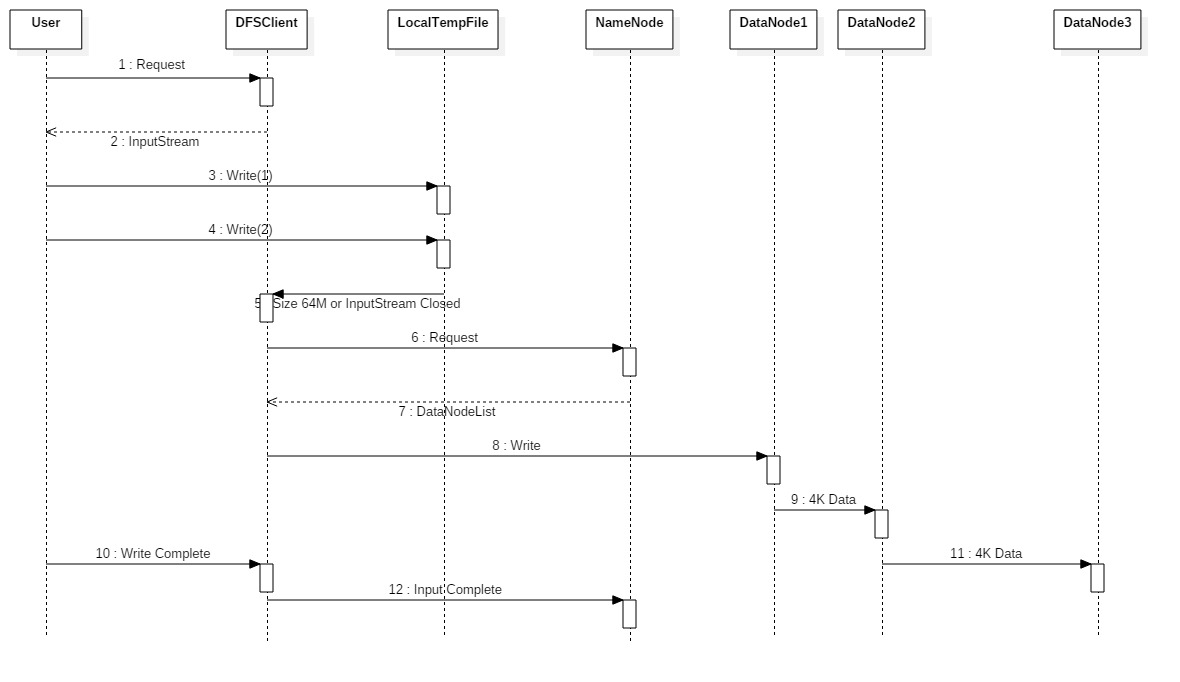
\includegraphics[width=1\linewidth]{HDFSInputTime}
            \caption{一个简单的HDFS写入操作时序图}
            \label{fig:HDFS Input Time}
        \end{figure}


    \subsubsection{其他文件系统实现}
        \begin{itemize}
            \item[*] HarFileSystem:归档文件系统
            \item[*] HttpFSFileSystem:基于Http协议的网络文件系统
            \item[*] HttpsFSFileSystem:基于Https协议的网络文件系统
            \item[*] FTPFileSystem:基于FTP文件传输协议的文件系统
        \end{itemize}


%% 结束
\endinput
%% abstractfilesystem
\section{Abstract File System}

图 \ref{fig:architecture} 是这个类的层次结构图。
\begin{figure}
\centering
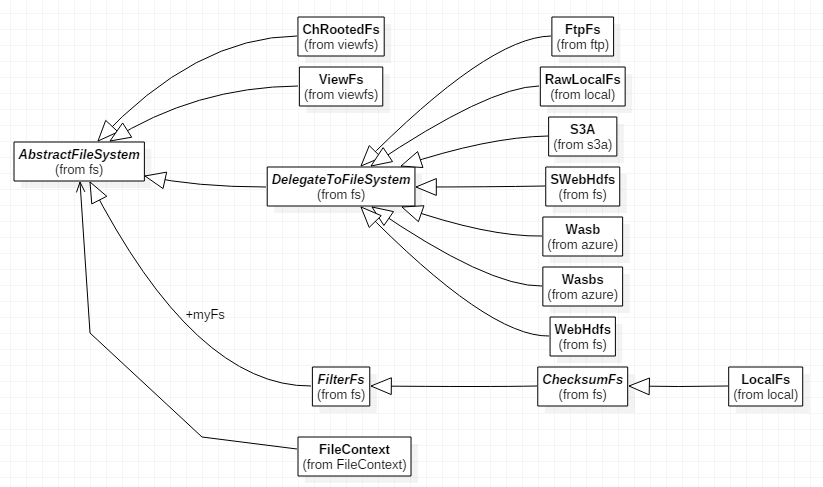
\includegraphics[width=1\linewidth]{UML/abstractfilesystem/architecture.PNG}
\caption{Abstract File System 的层次结构图}
\label{fig:architecture}
\end{figure}

\subsection{AbstractFileSystem}
Abstract File System类是一个抽象类,为Hadoop文件系统的实现者提供了一个接口(类似于Unix的VFS)。应用程序不访问此类,而是使用FileContext 访问所有文件系统中的文件。传递给AbstractFileSystem的路径名可以是与“this”文件系统(即相同的方案和权限)匹配的完全限定URI,或者假定相对于“this”文件系统的根目录的Slash相对名称。

\subsubsection{AbstractFileSystem类图}
图 \ref{fig:abstractFileSystem1}  \ref{fig:abstractFileSystem2} 是这个类的UML类图。

\begin{figure}
\centering
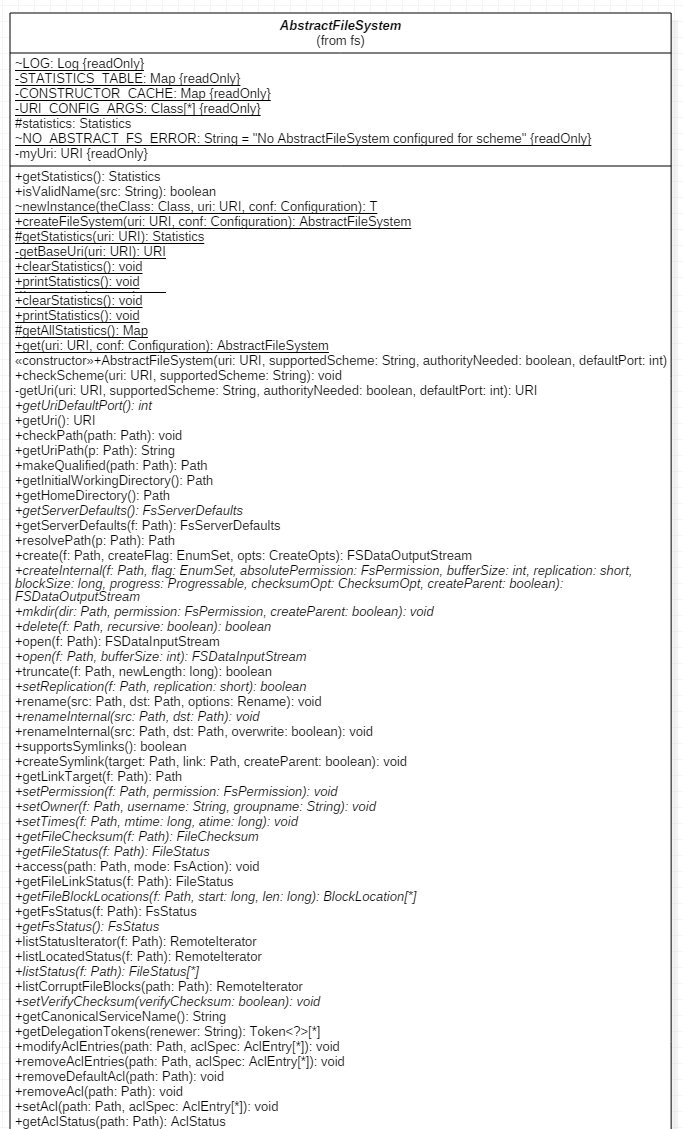
\includegraphics[width=1\linewidth]{UML/abstractfilesystem/abstractFileSystem1.PNG}
\caption{Abstract File System 的UML类图1}
\label{fig:abstractFileSystem1}
\end{figure}

\begin{figure}
\centering
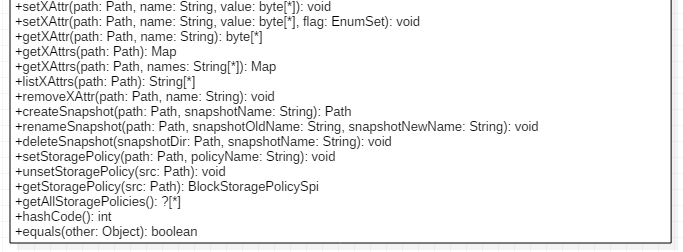
\includegraphics[width=1\linewidth]{UML/abstractfilesystem/abstractFileSystem2.PNG}
\caption{Abstract File System 的UML类图2}
\label{fig:abstractFileSystem2}
\end{figure}
从类图中我们可以看到,该类有对文件系统的基本操作。它与FileSystem有很多同名的方法,这些方法完成相同的功能,比如create,open,delete等等。getstatistics方法对于给定的文件系统获取统计数据。getinitialworkingdirectory方法获取文件系统初始工作目录。还有一些获取扩展属性的方法。

\subsubsection{get方法}
get方法是用于创建文件系统的主要工厂方法,获取uri的scheme和authority。uri的scheme确定一个配置属性名称fs.abastractfilesysytme.scheme.impl,将uri 和conf传递给createfilesystem函数。然后newInstance返回一个AbstractFileSystem的对象。
\begin{java}
  public static AbstractFileSystem get(final URI uri, final Configuration conf)
      throws UnsupportedFileSystemException {
    return createFileSystem(uri, conf);
  }

    /**
   * Create a file system instance for the specified uri using the conf. The
   * conf is used to find the class name that implements the file system. The
   * conf is also passed to the file system for its configuration.
   */
  public static AbstractFileSystem createFileSystem(URI uri, Configuration conf)
      throws UnsupportedFileSystemException {
    final String fsImplConf = String.format("fs.AbstractFileSystem.%s.impl",
        uri.getScheme());

    Class<?> clazz = conf.getClass(fsImplConf, null);
    if (clazz == null) {
      throw new UnsupportedFileSystemException(String.format(
          "%s=null: %s: %s",
          fsImplConf, NO_ABSTRACT_FS_ERROR, uri.getScheme()));
    }
    return (AbstractFileSystem) newInstance(clazz, uri, conf);
  }
\end{java}






\subsection{DelegateToFileSystem}
代理类是对各个具体的文件系统进行封装。抽象文件系统与fs不不同的是,fs的文件系统基本都是fs的直接子类。而在abstractfilesystem中很多文件系统都由delegatetofilesystem 代理。这些被代理的文件系统功能基本相同,实现只有些微的区别。
\subsubsection{DelegateToFileSystem类图}
图 \ref{fig:DelegateToFileSystem} 是这个类的UML类图。
\begin{figure}
\centering
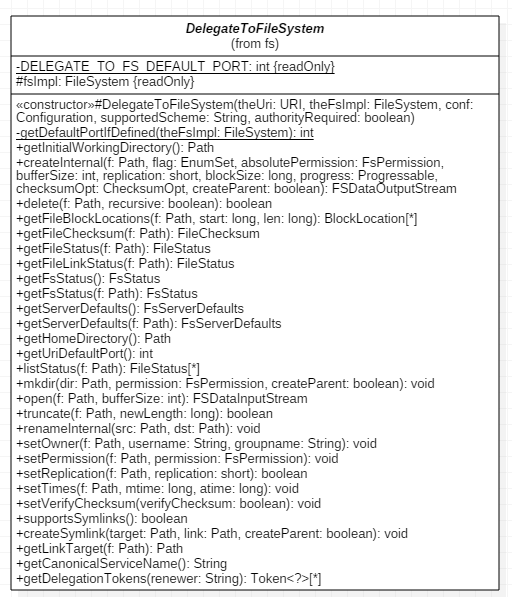
\includegraphics[width=1\linewidth]{UML/abstractfilesystem/DelegateToFileSystem.PNG}
\caption{DelegateToFileSystem的UML类图}
\label{fig:DelegateToFileSystem}
\end{figure}

\subsubsection{fsImpl}
在DelegateToFileSystem类中,有一个FileSystem类型的属性protected final FileSystem fsImpl,DelegateToFileSyste类的初始化要依靠这个属性。
\begin{java}
protected DelegateToFileSystem(URI theUri, FileSystem theFsImpl,
      Configuration conf, String supportedScheme, boolean authorityRequired)
      throws IOException, URISyntaxException {
    super(theUri, supportedScheme, authorityRequired,
        getDefaultPortIfDefined(theFsImpl));
    fsImpl = theFsImpl;
    fsImpl.initialize(theUri, conf);
    fsImpl.statistics = getStatistics();
  }
\end{java}

\subsubsection{S3A}
S3:Amazon S3(Simple Storage Service)是一种数据存储服务。
S3a:自Hadoop2.7以后运用的是s3a,s3a可支持较大的文件,具有更高的性能。替代以前的s3n.
构造函数中的new S3AFileSystem()是通过DelegateToFileSystem 中的FileSystem类型的属性完成的。
\begin{java}
/**
 * S3A implementation of AbstractFileSystem.
 * This impl delegates to the S3AFileSystem
 */
public class S3A extends DelegateToFileSystem{

  public S3A(URI theUri, Configuration conf)
          throws IOException, URISyntaxException {
    super(theUri, new S3AFileSystem(), conf, "s3a", false);
  }

  @Override
  public int getUriDefaultPort() {
    return Constants.S3A_DEFAULT_PORT;
  }
}
\end{java}

\subsubsection{RawLocalFs}
RawLocalFs是不带校验和的原生本地文件系统。
\begin{java}
/**
 * The RawLocalFs implementation of AbstractFileSystem.
 *  This impl delegates to the old FileSystem
 */

public class RawLocalFs extends DelegateToFileSystem {

  RawLocalFs(final Configuration conf) throws IOException, URISyntaxException {
    this(FsConstants.LOCAL_FS_URI, conf);
  }

  /**
   * This constructor has the signature needed by
   * {@link AbstractFileSystem#createFileSystem(URI, Configuration)}.
   */
  RawLocalFs(final URI theUri, final Configuration conf) throws IOException,
      URISyntaxException {
    super(theUri, new RawLocalFileSystem(), conf,
        FsConstants.LOCAL_FS_URI.getScheme(), false);
  }

  //......
}
\end{java}

\subsubsection{WebHdfs}
提供对HDFS的安全读写访问的文件系统,它利用的是http协议。旨在替代HFTP和HSFTP。hftp是在http上提供对hdfs只读访问的文件系统,虽然其名称为hftp但它与ftp无关。
\begin{java}
/**
 * AbstractFileSystem implementation for HDFS over the web.
 */
public class WebHdfs extends DelegateToFileSystem {

  public static final String SCHEME = "webhdfs";

  /**
   * This constructor has the signature needed by
   * {@link AbstractFileSystem#createFileSystem(URI, Configuration)}
   *
   * @param theUri which must be that of webhdfs
   * @param conf   configuration
   * @throws IOException
   */
  WebHdfs(URI theUri, Configuration conf)
      throws IOException, URISyntaxException {
    super(theUri, createWebHdfsFileSystem(conf), conf, SCHEME, false);
  }

  /**
   * Returns a new {@link WebHdfsFileSystem}, with the given configuration.
   */
  private static WebHdfsFileSystem createWebHdfsFileSystem(Configuration conf) {
    WebHdfsFileSystem fs = new WebHdfsFileSystem();
    fs.setConf(conf);
    return fs;
  }
}
\end{java}


\subsection{FilterFs}
一个FilterFs包含一些作为基本文件系统的其它的文件系统,会提供数据转换等附加功能。这个类FilterFs本身就是简单的覆盖所有版本的AbstractFileSystem 的方法,将所有请求传递给包含的文件系统的子类。FilterFs可以进一步覆盖这些方法中的一些,也可以提供其他方法和域。FilterFs类中拥有一个AbstractFileSystem类型的属性myFs。FilterFs 将其作为基本的文件系统。FilterFs 类几乎将所有重写的方法交给了其内部保存的myFs 来处理。但在交给myFs 处理之前,自己可以做一些处理,以此来实现过滤。
\begin{java}
public abstract class FilterFs extends AbstractFileSystem {
  private final AbstractFileSystem myFs;

  protected AbstractFileSystem getMyFs() {
    return myFs;
  }

  protected FilterFs(AbstractFileSystem fs) throws URISyntaxException {
    super(fs.getUri(), fs.getUri().getScheme(), false, fs.getUriDefaultPort());
    myFs = fs;
  }

  @Override
  public Statistics getStatistics() {
    return myFs.getStatistics();
  }

  @Override
  public Path makeQualified(Path path) {
    return myFs.makeQualified(path);
  }

  @Override
  public Path getInitialWorkingDirectory() {
    return myFs.getInitialWorkingDirectory();
  }
  //......
\end{java}


\subsection{ChecksumFs}
它提供了一个Checksumed Fs的基本实现,为每个原始文件创建一个校验和文件。在客户端生成并验证校验和。


\subsection{LocalFs}
LocalFs是ChecksumFs的实现,在LocalFs的构造函数中,实际上new了一个RawLocalFs。

\begin{java}
public class LocalFs extends ChecksumFs {
  LocalFs(final Configuration conf) throws IOException, URISyntaxException {
    super(new RawLocalFs(conf));
  }

  /**
   * This constructor has the signature needed by
   * {@link AbstractFileSystem#createFileSystem(URI, Configuration)}.
   */
  LocalFs(final URI theUri, final Configuration conf) throws IOException,
      URISyntaxException {
    this(conf);
  }
}
\end{java}



\subsection{FileContext}
\subsubsection{FileContext类图}
FileContext类为Hadoop文件系统的用户提供了一个接口。 它暴露了许多文件系统操作,例如创建,打开,列表。
图 \ref{fig:FileContext1} \ref{fig:FileContext2}是这个类的UML类图。
\begin{figure}
\centering
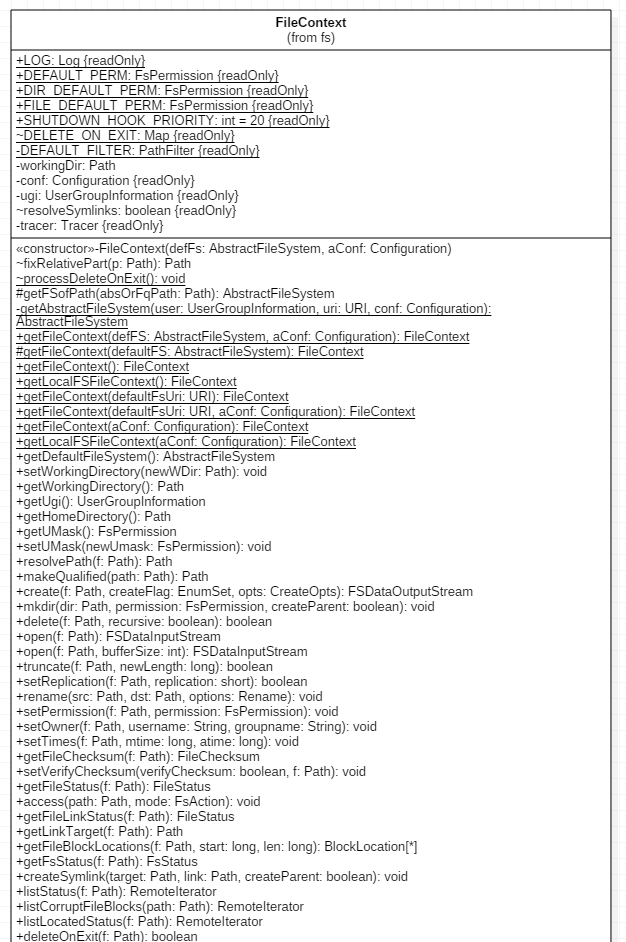
\includegraphics[width=1\linewidth]{UML/abstractfilesystem/FileContext1.PNG}
\caption{FileContext的UML类图1}
\label{fig:FileContext1}
\end{figure}

\begin{figure}
\centering
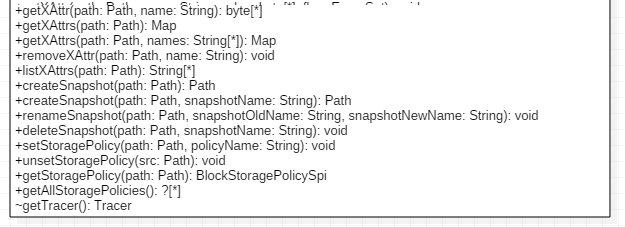
\includegraphics[width=1\linewidth]{UML/abstractfilesystem/FileContext2.PNG}
\caption{FileContext的UML类图2}
\label{fig:FileContext2}
\end{figure}

\subsubsection{getFileContext}
FileContext 由默认文件系统、工作目录和umask 定义。获得一个FileContext可以使用FileContext的静态方法:getFileContext();getLocalFSFileContext()
getFileContext有多重重载的形式。
\begin{quote}
示例1:使用从\verb|$HADOOP_CONFIG/core.xml|读取的默认配置。未指定的值来自发行版jar中的core-defaults.xml。
myFContext = FileContext.getFileContext();//使用默认配置//具有默认的FS
myFContext.create(path,…);
myFContext.setWorkingDir(路路径);
myFContext.open(path,…);…


示例2:获取具有特定URI的FileContext作为默认FS
myFContext = FileContext.getFileContext(URI);
myFContext.create(path,…);
\end{quote}

\subsubsection{Path Names}
Hadoop文件系统支持URI名称空间和URI名称。这使得要使用完全限定URI引用的多种类型的文件系统。
两个常见的Hadoop文件系统实现是
本地文件系统:file:/// path
HDFS文件系统:hdfs:// nnAddress:nnPort / path

Hadoop文件系统还支持URI之外的其他命名方案。
Hadoop具有默认文件系统的概念,这意味着默认URI方案和权限。这使得斜线相对名称有默认的FS,这对用户来说更为方便。
默认FS通常由用户环境设置,也可以手动指定。

Hadoop还支持工作目录相对的名称,它们是相对于当前工作目录(类似于Unix)的路径。工作目录可以在与默认FS不同的文件系统中。
因此,Hadoop路径名称可以指定为以下之一:
一个完全限定的URI:scheme:// authority / path(例如, hdfs:// nnAddress:nnPort / foo / bar)
斜线相对名称:相对于默认文件系统的路径(例如, / foo / bar)
工作目录相对名称:相对于工作目录的路径(例如, foo / bar)
scheme(scheme:foo / bar)的相对路径是非法的。

\subsubsection{FileContext的属性}
FileContext是Unix中每个进程文件相关状态的模拟。它包含两个属性:
默认文件系统(用于解析斜杠相对名称)
umask(用于文件权限)
一般来说,这些属性是在用户的环境中从默认配置文件获得的。
在服务器端指定了进一步的文件系统属性。文件系统操作默认使用这些服务器端默认值,除非另有说明指定。
文件系统相关的服务器端默认值为:
主目录(默认为“/ user / userName”)
初始wd(仅适用于本地fs)
复制因子
块大小
缓冲区大小
encryptDataTransfer
校验和选项。 (checksumType和bytesPerChecksum)

\subsubsection{open}
FileContext 中的很多方法是用来取代FileSystem中的方法的。包括create,mkdir,delete,open,setReplication,rename,setPermission,setOwner,setTimes,getFileStatus,getFileLinkStatus,getLinkTarget,getFileBlockLocations 等方法在AbstractFileSystem 中都有对应的方法。这些方法的实现具有相同的形式。比如open 方法的代码如下:
\begin{java}
/**
   * Opens an FSDataInputStream at the indicated Path using
   * default buffersize.
   */
 public FSDataInputStream open(final Path f) throws AccessControlException,
      FileNotFoundException, UnsupportedFileSystemException, IOException {
    final Path absF = fixRelativePart(f);
    return new FSLinkResolver<FSDataInputStream>() {
      @Override
      public FSDataInputStream next(final AbstractFileSystem fs, final Path p)
        throws IOException, UnresolvedLinkException {
        return fs.open(p);
      }
    }.resolve(this, absF);
  }

  /**
   * Opens an FSDataInputStream at the indicated Path.
   */
  public FSDataInputStream open(final Path f, final int bufferSize)
      throws AccessControlException, FileNotFoundException,
      UnsupportedFileSystemException, IOException {
    final Path absF = fixRelativePart(f);
    return new FSLinkResolver<FSDataInputStream>() {
      @Override
      public FSDataInputStream next(final AbstractFileSystem fs, final Path p)
        throws IOException, UnresolvedLinkException {
        return fs.open(p, bufferSize);
      }
    }.resolve(this, absF);
  }
\end{java}
FileContext.open是通过调用AbstractFileSystem.open来实现的。

open操作的时序图示例:
图 \ref{fig:sequence} 是这个类的层次结构图。
\begin{figure}
\centering
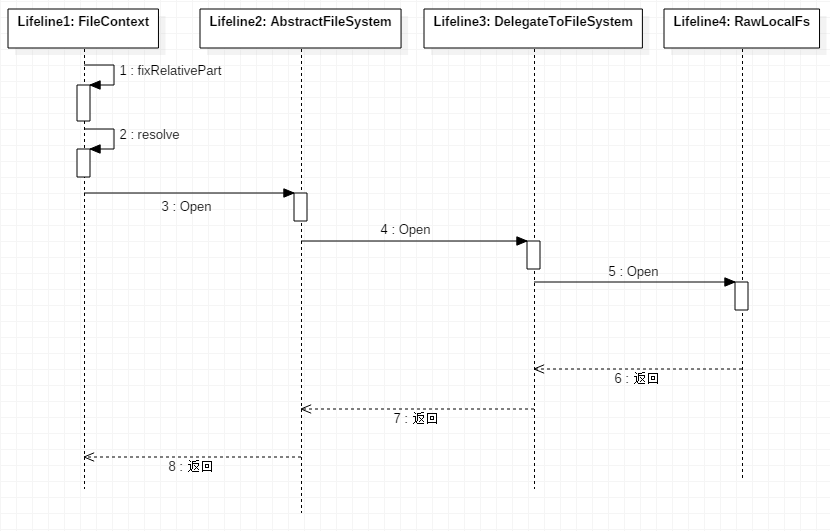
\includegraphics[width=1\linewidth]{UML/abstractfilesystem/sequence.PNG}
\caption{open操作的时序图}
\label{fig:sequence}
\end{figure}





%% 结束
\endinput
    %% 修复
    \section{针对批注的回答}
\label{sec:fix}

%% 批注一的回答

\subsection{批注一的回答}
\label{sec:fix:bl1}

Hadoop 是一个\textbf{分布式系统基础框架}。在将底层细节“屏蔽”的基础上,为用户提供开发分布式程序的基础设施,高效利用集群,及其计算、存储能力。
Hadoop 是由 \href{https://www.apache.org}{Apache}基金会所开发维护的分布式系统架构。核心部分由 HDFS 和 MapReduce 组成。
HDFS 提供了一个分布式的文件存储方式,提供了高容错性文件系统且可在低廉设备部署,同时相对具有较高的吞吐量。
%% 批注二

\subsection{批注二的回答}
\label{sec:fix:bl2}

HDFS 与 Linux 系统中的 VFS 相类似。首先在 Linux 系统中, VFS 是 \verb|Virtual File System| 的缩写。 VFS 解决掉的问题不是说针对某一个特定的文件系统的实现,或者
文件系统应该如何实现。VFS 做的是 抽象的描述出了一个文件系统提供,尤其是对上层提供的 API 接口或者是所具有的功能有哪些。简而言之,描述了一个对于更高层次的结构来说,文件系统长得什么样子。
HDFS 类似的提拱了一些“接口描述”,或者更加形象使用 Haskell 中的类型类进行“比喻”。

由此可见 HDFS 是依赖与底层的文件系统实现,然后向高层用户提供相关内容的访问。而底层文件系统则相对“依赖” HDFS 中描绘的接口,以规范自身。

HDFS 同时做的一件事情是:将不同的文件系统对接到一起。正如在 Linux 中,我们可以将 Ext4 文件系统下的文件复制到 exFAT 文件系统中, HDFS 也提供了类似的支持。
本身两种不同文件系统会具有比较大的差异,而 HDFS 做的是从文件系统A中拿出东西,在放到文件系统B中。
%% 批注三的回答

\subsection{批注三的回答}
\label{sec:fix:bl3}

这里的“本地”一词用来指代所在的操作系统中的文件系统的抽象层。
由于各类操作系统本身的特性,无论是那种操作系统,都需要一层“文件系统抽象层”来将不同的文件系统抽象出来。
这里的“本地”的意思就是使用这一层抽象层,而不是具体的文件系统
%% 批注四的回答

\subsection{批注四的回答}
\label{sec:fix:bl4}

针对第四个批注的内容,在回答之前首先需要介绍一下很多云服务提供商的文件存储服务。
诸如腾讯云,青云,阿里云,亚马逊云,微软的Azure等云服务提供商,会提供多种服务,包括云主机的业务,和文件存储的服务。
通常情况下,储存数据的选择有很多,可以使用数据库,无论是传统的数据库还是 NoSQL 的数据库,同时还可以选择“硬盘”。
云服务上提供的“硬盘”,通常有两种,一种是提供给虚拟主机使用的硬盘,与物理主机使用的硬盘类似。此外还有另一种,
存储服务,由于前者并不适用于很多业务场景,诸如一份大文件为需要被很多节点使用,所以大多是提供云服务的服务商,同时提供了
对象存储服务。下面是摘录自腾讯云\textit{对象存储服务}页面的一段介绍内容:
\begin{quote}
    对象存储(Cloud Object Storage)是面向企业和个人开发者提供的高可用,高稳定,强安全的云端存储服务。
    您可以将任意数量和形式的非结构化数据放入COS,并在其中实现数据的管理和处理。COS支持标准的Restful API接口,
    您可以快速上手使用,按实际使用量计费,无最低使用限制。
\end{quote}
很多提此类服务供商处于一定技术原因,会限制单个存储对象的大小。而这里的存储对象和传统的文件有类似的地方但是概念也不大相同。
在最新的亚马逊的官方文档中,存储服务已经更名为 \verb|Amazon Elastic File System|,EFS 为缩写。 在 EFS 的 FAQ 并没有见到
提及任何大小限制,同时有如下一段描述:
\begin{quote}
    Amazon EFS 文件系统可以自动将数据容量从 GB 级扩展到 PB 级,无需预置存储。
\end{quote}

简单概括,这个文件系统就是将对象存储服务的 API 封装成类似与文件系统的东西,也就是原生的。5G 大小的限制则是来自
对象存储服务的限制,目前应该是已经取消。
%% 批注五的回答

\subsection{批注五的回答}
\label{sec:fix:bl5}

批注五指向的,所谓的“破坏器”,应该是英文\verb|destructor| 的生硬翻译。通常会有一组英文叫做 construct 与 destruct,
在 C++ 中可以翻译为构造器与析构器。在此处,推测是由于 \lstinline|FilterInputStream| 这里采用了装饰器模式,所以所谓的
破坏其应该是 “construct” 的逆向过程用于装饰。
%% 批注六的回答

\subsection{批注六的回答}
\label{sec:fix:bl6}

管道作为一种数据传送接口来说一般需要一个入口与一个出口,就像水管一样, 一头流入同时一头流出。\lstinline|PipedOutputStream| 作为一个数据源,需要有一个输出的地方,所以可以
与 一个\lstinline|FilterInputStream| 对接然后获取数据。例如将\lstinline|PipedOutputStream|与\lstinline|PipedInputStream|组合到一起形成一个管道。
%% 批注七的回答

\subsection{批注七的回答}
\label{sec:fix:lb7}

\lstinline|SequenceInputStream| 提供的功能是将多个 \lstinline|InputStream| 转换成了一个单独的 \lstinline|InpuStream| 或者是 \lstinline|Enumeration|,
转换的到的这一个 \lstinline|InputStream| 可以与 \lstinline|FilterInputStream| “组合”,就如同通常的的使用 \lstinline|FilterInputStream| 的是时候使用 \lstinline|InputStream|
方式是一样的。 
%% 批注八的回答

\subsection{批注八的回答}
\label{sec:fix:lb8}

这里的问的内容与批注六的内容是一样的,只是换成了 输出流,其他都一样。
%% 批注九的回答

\subsection{批注九的回答}
\label{sec:fix:bl9}

\lstinline|DataInputStream| 继承了 \lstinline|FilterInputStream|,其中 后者是使用 \lstinline|InputStream| 中的 \lstinline|read| 函数,封装了一些新的函数,
提供更多的功能。而 \lstinline|DataInputStream| 继承后者之后,也是使用 \lstinline|InputStream| 并封装了一些新的函数。其中在这两个类中那个类型为 \lstinline|InputStream|
的属性名称正是叫 \lstinline|in|。

%%批注十的回答

\subsection{批注十的回答}
\label{sec:fix:bl10}

\lstinline|FileSystem| 的图,可以参见 部分中的图片 。
%% 批注十一的回答
\subsection{批注十一的回答}
\label{sec:fix:bl11}

\lstinline|Closeable| 这个接口从字面意义上来讲,大致是“可以关闭的”的意思。一般指一些需要进行关闭的操作,来关闭、释放一些系统资源。
例如 文件流,Socket 套接字,管道,硬件等打开时系统会为之分配一些资源,然后需要在不要的时候关闭,一方面释放资源,另一方面停止占用。
这样设计能比较不错的管理资源。

%% 结束
\endinput


\end{document}

